\documentclass[a5paper, twoside]{article}
\usepackage{fullpage}
\usepackage[czech]{babel}
\usepackage{amsfonts}
\usepackage[a5paper,margin=25pt]{geometry}
\usepackage{fontspec}
\usepackage{sectsty}
\usepackage{xcolor}
\usepackage{pagecolor}
\usepackage{afterpage}
\usepackage[many]{tcolorbox}
\usepackage{setspace}
\usepackage{multicol}
\usepackage{enumitem}
\usepackage[compact]{titlesec}
\usepackage{graphicx}
\usepackage{caption}
\usepackage{mdframed}
\usepackage{pdfpages}
\usepackage{pdflscape}

\graphicspath{{images/}}

\setlist[itemize]{noitemsep}

\pagenumbering{gobble}

\setstretch{1}
\titlespacing{\section}{0pt}{-3pt}{10pt}

\titleformat*{\section}{\LARGE\bfseries}

% definuj jaroška barvy
\definecolor{red}{cmyk}{0.15, 1, 0.85, 0}
\definecolor{blue}{cmyk}{0.89, 0, 0.12, 0.2}
\definecolor{green}{cmyk}{0.75, 0, 0.55, 0.3}
\definecolor{yellow}{cmyk}{0, 0.35, 0.75, 0.12}
\definecolor{darkblue}{cmyk}{0.88, 0.48, 0, 0.52}

% nastav jaroška fonty
\newfontfamily\Kapitan{Kapitan-Medium}
\setmainfont{ClearSans}

% nastav hodnoty pro hezké boxíky
\tcbset {
    colback = white,
    before skip = 0.2cm,
    after skip = 0.5cm
}

% barva pozadí, barva textu, text
\newcommand{\boxik}[3]{
  \begin{tcolorbox}[
    sharp corners,
    colback = #1,
    boxrule = 0pt,
    grow to left by = 25pt,
    grow to right by = 25pt,
    right = 22pt,
    left = 22pt%,
    %enlarge bottom by = -4pt
  ]
    \textcolor{#2}{#3}
  \end{tcolorbox}
}

% params: section title, background color, text color, grow to side by
\newcommand{\nadpis}[4]{
  \vspace*{-50pt}
  \begin{tcolorbox}[colback = #2, boxrule = 0pt, grow to left by = #4,  grow to right by = #4, arc=8pt, height = 40pt]
    \vspace*{5pt}
    \centering \section*{\textcolor{#3}{#1}}
  \end{tcolorbox}
}

\newcommand{\polonadpis}[4]{
  \vspace*{-50pt}
  \begin{tcolorbox}[colback = #2, boxrule = 0pt, grow to left by = #4,  grow to right by = #4, arc=8pt, height = 30pt]
    \vspace*{5pt}
    \centering \subsection*{\textcolor{#3}{#1}}
  \end{tcolorbox}
}

% params: subsection title, text color
\newcommand{\podnadpis}[2]{
  \subsection*{\textcolor{#2}{#1}}
}

%\newcommand{\pagenumberbox}[4]{
  %\vspace*{-60pt}
  %\hspace*{-185pt}
  %\begin{tcolorbox}[colback = #2, boxrule = 0pt, grow to left by = #4,  grow to right by = #4, arc=8pt, height = 20pt]
    %\vspace*{20pt}
    %\centering \textcolor{#3}{\textbf{\large{#1}}}
  %\end{tcolorbox}
%
%\newcommand{\rpagenumberbox}[4]{
%  \hspace*{150pt}
%  \begin{tcolorbox}[colback = #2, boxrule = 0pt, grow to left by = #4,  grow to right by = #4, arc=8pt, height = 20pt]
%    \centering \textcolor{#3}{\textbf{\large{#1}}}
%  \end{tcolorbox}
%}

\begin{document}
\begin{titlepage}
	\newgeometry{margin=0pt}
	\pagecolor{red}
	\begin{center}
		\vspace*{\fill}

		\textcolor{white}{\fontsize{60}{60} \Kapitan Průvodce\\\vspace{0.2em}prváka}

		\vspace*{\fill}
		\textcolor{white}{\fontsize{20}{20} \Kapitan Jaroška}

		\vspace{0.5em}

		\boxik{blue}{white}{\centering \fontsize{15}{15} \Kapitan \textcolor{white}{2024/2025}}

		\vspace{3em}

	\end{center}
\end{titlepage}
\pagecolor{white}


% mapa školy-
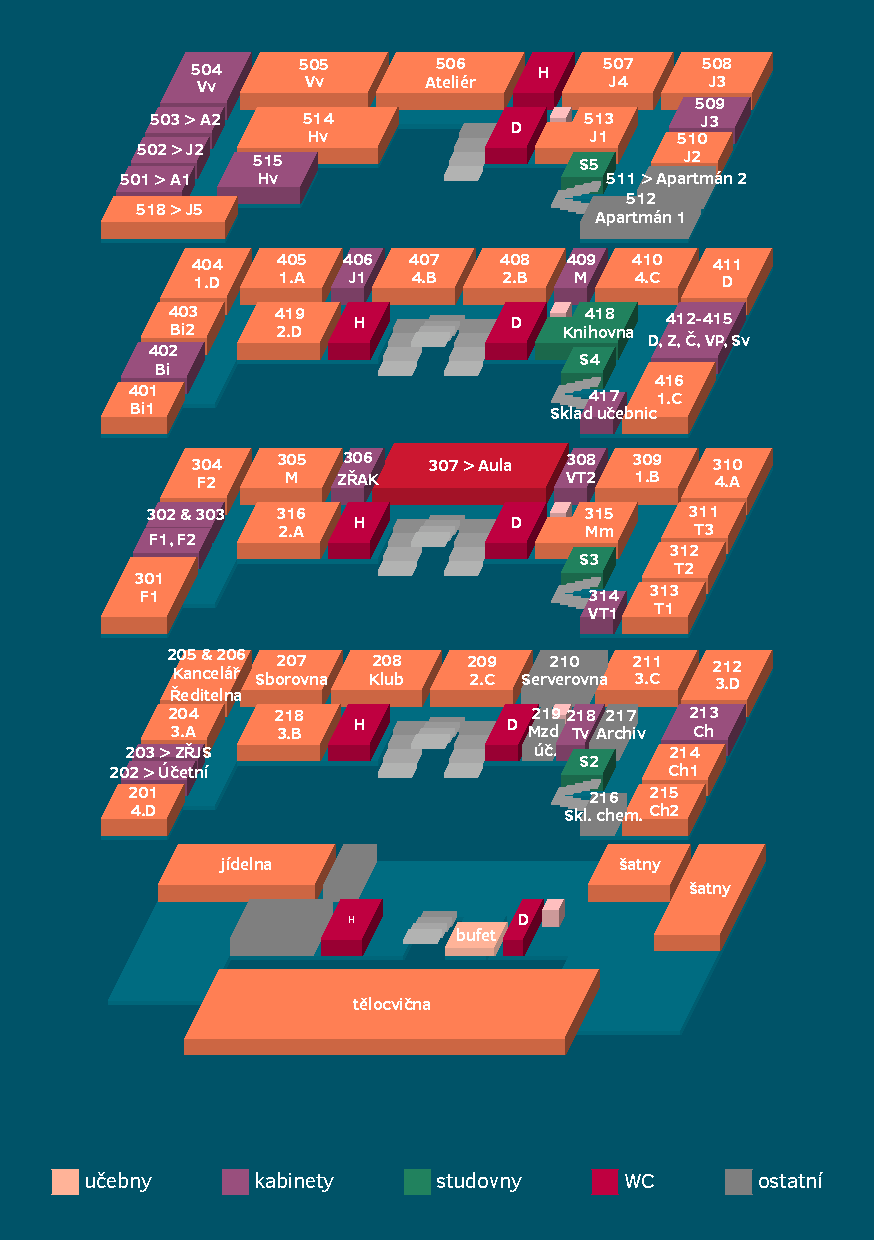
\includepdf[pages=-]{mapa_skoly.pdf}
\newpage

\setcounter{page}{1}
% kabinety
\noindent
\newpagecolor{darkblue}

\nadpis{SEZNAM KABINETŮ}{white}{darkblue}{-3.25cm}

\textcolor{white}{
  \noindent \begin{tabular}{l l l}
    Kabinet hala & 1. podlaží & Zvolská \\
    Kabinet AŠSK & 1. podlaží & Jadvidžák, Stupka \\
    Finanční účetní & 202 & Polachová \\
    Kabinet ZŘ & 203 & Sítařová \\
    Kancelář & 205 & Jemna \\
    Ředitelna & 206 & Nečas \\
    Server & 210 & Rádl \\
    Chemie & 213 & Brančová, Kyasová, Plavčanová, Vašíčková \\
    Tělená výchova & 218 & Stupka, Doležal, Liškutín, Marková D., \\
    & & Štarhová \\
    Mzdová účetní & 219 & Šuléřová \\
    Fyzika 1 & 302 & Přikryl, Glozar, Kučera, Sekerka \\
    Fyzika 2 & 303 & Lacinová, Ježek, Řehák \\
    Kabinet ZŘ & 306 & Kobza \\
    Výpočetní technika 2 & 308 & Horáková N., Hájková V., Krejčí T. \\
    Výpočetní technika 1 & 314 & Blaha, Krejčí P. \\
    Biologie & 402 & Kubištová, Kupčík, Vařejka \\
    Jazyky 1 & 406 & Zvolská, Chovancová, Literáková \\
    Matematika & 409 & Šťastná, Boucník, Juránek, Trnka \\
    Dějepis, zeměpis & 412 & Šlesingerová, Maříková \\
    Čeština & 413 & Marková L., Mrkosová \\
    Kabinet VP & 414 & Borošová, Nováková M. \\
    Společenské vědy & 415 & Pospíšil, Bučková, Horáková J. \\
    Sklad učebnic & 417 & Horák, Zerhau \\
    Knihovna & 418 & Pleva, Hudeček, Tillová, Urban \\
    Angličtina 1 & 501 & Smělíková Pilátová, Kallus Brychová \\
    Jazyky 2 & 502 & Jugasová, Sedlinská \\
    Angličtina 2 & 503 & Kubitová, Zubíčková \\
    Výtvarná výchova & 504 & Havlíčková, Hubáček, Nobbs, O'Malley \\
    Jazyky 3 & 509 & Adámková, Clausová, Novotná, Vomelová \\
    Hudební výchova & 515 & Ambrozová, Ptáčková, Řihánková
  \end{tabular}
  }
  \vfill
  \noindent\textcolor{white}{\textbf{Poznámka.} Jak si můžeš všimnout, na naší škole nemáme \textit{patra}, ale \textit{podlaží}. Ve zkratce: když vejdeš dveřmi z ulice, jsi v nultém patře (v přízemí -- tento přístup razí informatici), ale v 1. podlaží. \\
  Navíc, každé dveře mají svoje číslo. Třeba 4.A -- 310. To má svou určitou logiku: první číslice z trojice značí podlaží a další dvě značí polohu na daném podlaží tak, že 01 je nejvíc vzadu vlevo v pohledu od schodů a s každou další místností směrem doprava roste o jedna. Pokud nebudeš vědět, kde je jaká učebna, rozklikni si v rozvrhu v EduPage i její číslo a trefíš tam i poslepu!}
\newpage
\newpagecolor{white}

\nadpis{JAK TO U NÁS CHODÍ}{red}{white}{-3cm}
\noindent \podnadpis{DĚLENÍ TŘÍD}{red}
\begin{itemize}[leftmargin=10pt]
	\item \textcolor{red}{\textbf{X.A}} --  \textbf{matematicky zaměřená třída}, většina studentů už jde z tzv. nižšího gymnázia na Příční ulici (prima až kvarta), na vyšším se k nim následně připojí pár dalších studentů
	\item \textcolor{red}{\textbf{X.B}} -- \textbf{všeobecná třída}, taky přicházejí z nižšího gymnázia
	\item \textcolor{red}{\textbf{X.C}} -- \textbf{všeobecná třída}, druhý cizí jazyk je volitelný: vítězí většinou němčina, ale
	      k dispozici je i španělština, francouzština a ruština
	\item \textcolor{red}{\textbf{X.D}} -- \textbf{všeobecná třída}, druhý cizí jazyk může být pouze němčina
\end{itemize}
\podnadpis{IT}{red}
\begin{itemize}[leftmargin=10pt]
	\item na začátku školního roku dostane každý/á student/ka svoje přihlašovací údaje k~\textbf{elektronické třídnici EduPage}
	\item také existuje trochu jiné ID, díky kterému se budeš moct \textbf{přihlašovat v informatice} k počítačům na školní síti a taky na \textbf{školní wifinu}
\end{itemize}

\parskip

\boxik{red}{white}{\begin{itemize}[leftmargin=10pt]
    \item S \textbf{připojováním osobních notebooků} na školní wifi to bývalo v minulosti trochu složitější. Naštěstí v minulém školním roce naše zastaralá síť přošla značnými úpravami, takže už by to teď \textbf{neměl být problém}. Stačí se přihlásit na síť \textit{JAROSKA\_S} se \textbf{stejným jménem a heslem}, jako se přihlašuješ v informatice. Pokud si heslo na počítač změníš, změní se ti i heslo na wifi! V případě, že něco nebude fungovat, \textbf{zajdi za panem profesorem Blahou} (jehož kabinet si můžeš najít na plánku školy) a popros ho o pomoc.
  \end{itemize}
}

\begin{itemize}[leftmargin=10pt]
	\item  škola nám laskavě poskytuje \textbf{studentský server Penguin} (\textit{penguin.jaroska.cz}), slouží primárně pro projekty studentů/ek; pokud plánuješ třeba uspořádat školní akci, potřebuješ server pro svoji ZP a nebo jen sháníš úložiště/pískoviště pro svoje vyžití, \textbf{nechceš platit hosting a nevadí ti trochu starší způsob přístupu k souborům}, obrať se na profesory informatiky, kteří tě pak můžou nasměrovat na \textbf{odpovědné správce serveru}; zpravidla to bývá \textbf{někdo ze studentstva}
\end{itemize}

\podnadpis{ŠKOLNÍ MAILY}{red}
\begin{itemize}[leftmargin=10pt]
	\item Každý profesor má založený \textbf{svůj školní mail ve tvaru} \textit{prijmeni@jaroska.cz} (až na výjimky, jako třeba pan profesor Řehák: \textit{czehi@jaroska.cz}), na kterém ho můžeš kontaktovat. S tímhle mailem se většinou nespleteš, ale pro sichr je vždycky lepší se přímo dotyčného profesora \textbf{zeptat, jestli náhodou nemá mail na jiné doméně}, kterou používá častěji -- díky tomu můžeš dostat rychlejší odpověď.
	\item  Taky ti sem dáme pár důležitých mailů, které by se ti mohly hodit:
  \begin{itemize}[leftmargin=0pt]
    \item ředitel: \textcolor{red}{\textbf{necas@jaroska.cz}}
    \item zástupce (ten, co řeší vnitroškolní věci): \textcolor{red}{\textbf{akob@jaroska.cz}}
    \item statutární zástupkyně (třeba na záležitosti s ISICem): \textcolor{red}{\textbf{sitarova@jaroska.cz}}
    \item hospodářka (té napiš při problémech se systémem obědů): \textcolor{red}{\textbf{turcanu@jaroska.cz}}
  \end{itemize}
\end{itemize}

\newpage

\polonadpis{I. Jak to u nás chodí}{red}{white}{-4.1cm}

\podnadpis{VOLITELNÉ PŘEDMĚTY}{red}

\noindent V rámci možností (a našich osnov) jdeme s dobou -- \textbf{pro 3. a 4. ročník si tedy
	můžeš} (respektive musíš) \textbf{vybrat volitelné předměty}. Výčet níže ber s rezervou
(může se cokoli změnit, některé předměty mohou přibýt nebo ubýt). V případě
nízkého zájmu se rovněž \textbf{některé předměty nemusejí otevřít}, ale v posledních
letech se snažíme dělat vše pro to, aby byl každý spokojen.

\begin{multicols}{2}
	\noindent \textcolor{red}{\textbf{1. a 2. volitelný předmět} (matematická třída bere jeden, všeobecné berou dva; vybírá se na konci druháku na dva roky)}
	\begin{itemize}
		\item 3. cizí jazyk (N, Fr, Š, Ru)
		\item Cambridge Exam Preparation
		\item Cvičení z biologie a chemie
		\item Cvičení z matematiky a fyziky
		\item Dějiny umění
		\item Deskriptivní geometrie
		\item Ekonomika
		\item Informatika a programování
		\item Konverzace ve 2. cizím jazyce
		\item Latina
		\item Molekulární biologie
	\end{itemize}

	\noindent \textcolor{red}{\textbf{3. a 4. volitelný předmět} (matematická třída bere jeden, všeobecné berou dva; vybírá se na konci třeťáku pro maturitní ročník)}
	\begin{itemize}
		\item Biologie 2
		\item Business English
		\item Dějepis 2
		\item Finanční gramotnost
		\item Fyzika 2 (4.B, C nebo D)
		\item Chemie 2
		\item Informatika a programování 2
		\item Konverzace ve 2. cizím jazyce
		      (pokud nezvolena dříve)
		\item Matematika 2 (4.B, C nebo D)
		\item Moderní dějiny
		\item Zeměpis 2
	\end{itemize}

	\vfill\null

	\columnbreak

	\noindent \textcolor{red}{\textbf{Maturitní semináře} (bereš dva, vybírají se na maturitní ročník)}
	\begin{itemize}
		\item S. z biologie
		\item S. z českého jazyka a literatury
		\item S. z dějepisu
		\item S. z deskriptivní geometrie (při
		      dřívějším zvolení běžné Deskriptivy)
		\item S. z ekonomiky (při dřívějším zvolení předmětu Ekonomika)
		\item S. z fyziky
		\item S. z chemie
		\item S. z informatiky
		\item S. z matematiky (pro 4.B, C a D)
		\item S. z matematických aplikací (4.A)
		\item S. ze společenských věd
		\item S. ze zeměpisu
	\end{itemize}

	\noindent \textcolor{red}{\textbf{Sport} (bereš jeden, vybírá se na konci třeťáku pro maturitní ročník)}
	\begin{itemize}
		\item Fotbal
		\item Plavání
		\item Posilování
		\item Squash
		\item Tanec
		\item Volejbal
	\end{itemize}

	\begin{tcolorbox}[colback=red,boxrule=0pt, sharp corners]
		\textcolor{white}{\footnotesize \textbf{Poznámky.}
			Některé předměty jsou označeny pro třídy X.A apod. Osnovy matematické a všeobecné třídy se trochu liší, a proto jim musí být
			uzpůsoben i repertoár volitelných předmětů.\\
			Výčet nemusí být kompletní:
			neustále se snažíme vymýšlet nové smysluplné
			předměty -- hlavně do čtvrťáku. A některé ze
			seznamu se vůbec nemusejí otevřít.
      }

		\hfill
	\end{tcolorbox}
\end{multicols}

\newpage

\polonadpis{I. Jak to u nás chodí}{red}{white}{-4.1cm}

\podnadpis{ŠKOLNÍ KANCELÁŘ}{red}

Na vyřizování formalit tu máme \textbf{školní kancelář}. \textbf{Najdeš ji ve druhém patře}, jako
navigaci můžeš použít schéma školy na začátku \textcolor{black}{\Kapitan Průvodce prváka}.
Využiješ ji hlavně na:
\begin{itemize}[leftmargin=10pt]
	\item \textbf{potvrzení o studiu} -- na šalinkartu nebo úlevy na daních,
	\item \textbf{čip do jídelny} -- o tom ti víc řekneme v odstavci Jídelna (str. 9),
	\item \textbf{čip k výtahu} -- pokud si přivodíš úraz v naší (krásné!) tělocvičně,
	\item \textbf{ztráty a nálezy} -- buď tady, nebo na vrátnici,
	\item \textbf{hlášení úrazů} -- abychom ti mohli třeba vyjednat odškodné.
\end{itemize}

\podnadpis{JEŽDĚNÍ VÝTAHEM}{red}
\begin{minipage}{0.65\linewidth}
	\par Schody tu jsou pro každého, výtah ne úplně. Nějaký/á dobrák/ačka profesor/ka tě občas sveze, i když jsi mohoucí, ale je jich menšina (jak by to tady pak vypadalo), a~\textbf{proto se povolení na použití výtahu rozdávají až na základě nějakého relevantního zranění}.
  \par Podání žádosti probíhá tak, že \textbf{poprosíš svého třídního učitele / svou třídní učitelku o podepsaný formulář}, s tím budeš muset \textbf{skočit do kanceláře} (což se ti se zlomenou nohou možná bude dělat blbě), kde ti sdělí \textbf{tajný kód}, \textbf{který pak budeš muset říct profesoru Blahovi a na tvůj
		obědový čip ti nahraje kód na výtah} -- budeš tak mít už dva důvody ho neztratit.
\end{minipage}
\begin{minipage}{0.35\linewidth}
	\centering
	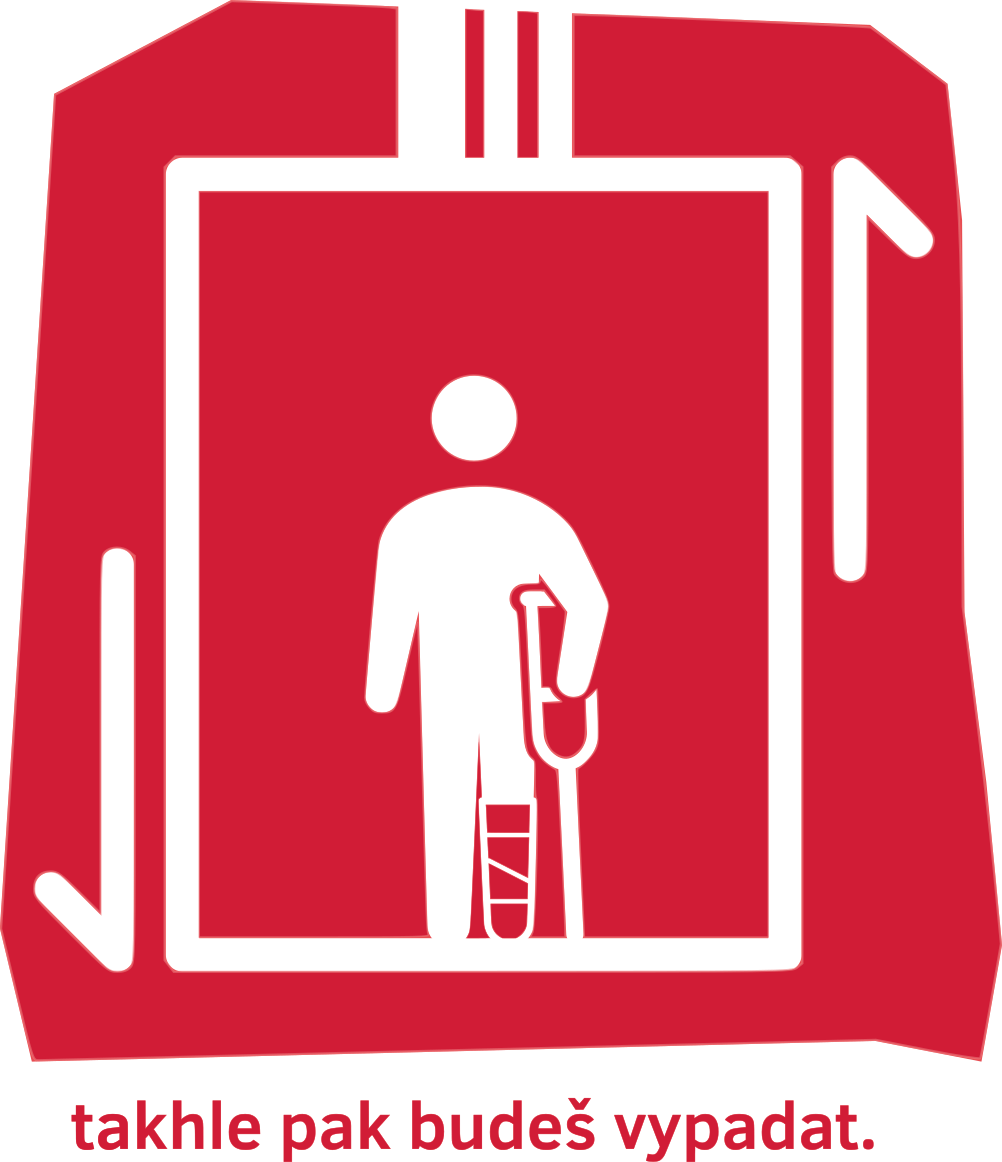
\includegraphics[width=0.90\linewidth]{vytah.png}
\end{minipage}
\vspace{0pt}\\
\noindent
Výtah samotný se pak používá tak, že se \textbf{prvně pípneš čipem na bílou krabičku
	vlevo od výtahových dveří a až pak si zmáčkneš tlačítko přivolání}. \\
Ve zkratce: nemohoucí a profesoři/profesorky jezdí výtahem, ostatní nejezdí (a nebo jezdí jen
velmi opatrně). Přejeme pěknou jízdu!

\parskip

\boxik{red}{white}{\textbf{Poznámka.} Ne že bys nejen nesměl/a jezdit zdravý/á výtahem, ono to taky dost dobře nejde. Bez oprávnění na čipu tě výtah prostě nebude poslouchat a nepřijede ti. Když už je mysteriózně otevřen na patře prázdný, nikdo ti asi nebude fyzicky bránit do něj naskočit a odjet -- ale pokud tě při tom načapá profesor/ka, který/á to nemá rád/a, dostaneš bídu. Takže bacha.}

\podnadpis{A CO ISIC?}{red}
Být studentem/studentkou je dřina, když ti to průvodčí nevěří. Za drobnou úplatu ti tu však samozřejmě \textbf{vystavíme studentský průkaz ISIC}. Stačí vyplnit žádost (kterou najdeš na {\bf jaroska.cz} v příslušné sekci, a nebo v kanceláři na stole), \textbf{předat ji paní zástupkyni Sítařové} a na její mail (\textbf{sitarova@jaroska.cz}) pošli reprezentativní \textbf{fotku} o rozlišení minimálně 300 x 360 px. Nechceme fotky naskenované z dokladů (ačkoli normální headshots jsou v pohodě), divně oříznuté, rozmazané nebo jinak nekvalitní.

\newpage

\polonadpis{I. Jak to u nás chodí}{red}{white}{-4.1cm}

\podnadpis{ŠKOLNÍ VÝLETY}{red}
Ačkoli nám do toho covid v posledních letech házel vidle, jezdíme i na výlety.
\textbf{V~každém ročníku tě čeká jeden} -- \textbf{tady je jejich přehled}.

\begin{itemize}[leftmargin=10pt]
	\item \textcolor{red}{\textbf{Prvák a druhák:}} \textbf{třídenní výlet}, který si volí třída, lze protáhnout i do víkendu
	\item \textcolor{red}{\textbf{Třeťák:}} každý rok jsou připraveny \textbf{čtyři sportovní kurzy}, ze kterých si každý student zvolí jeden: \textbf{vodácký kurz}, \textbf{vysokohorská turistika}, \textbf{zájezd do Chorvatska}, \textbf{windsurfing}
	\item \textcolor{red}{\textbf{Čtvrťák:}} \textbf{třídenní literárně-historická exkurze do Prahy}
\end{itemize}

\parskip

\boxik{red}{white}{
\begin{minipage}{\linewidth}
  \begin{minipage}{0.32\linewidth}
    \includegraphics[width=\linewidth]{tatry.jpg}
  \end{minipage}
  \hfill
  \begin{minipage}{0.32\linewidth}
    \includegraphics[width=\linewidth]{voda.png}
  \end{minipage}
  \hfill
  \begin{minipage}{0.32\linewidth}
    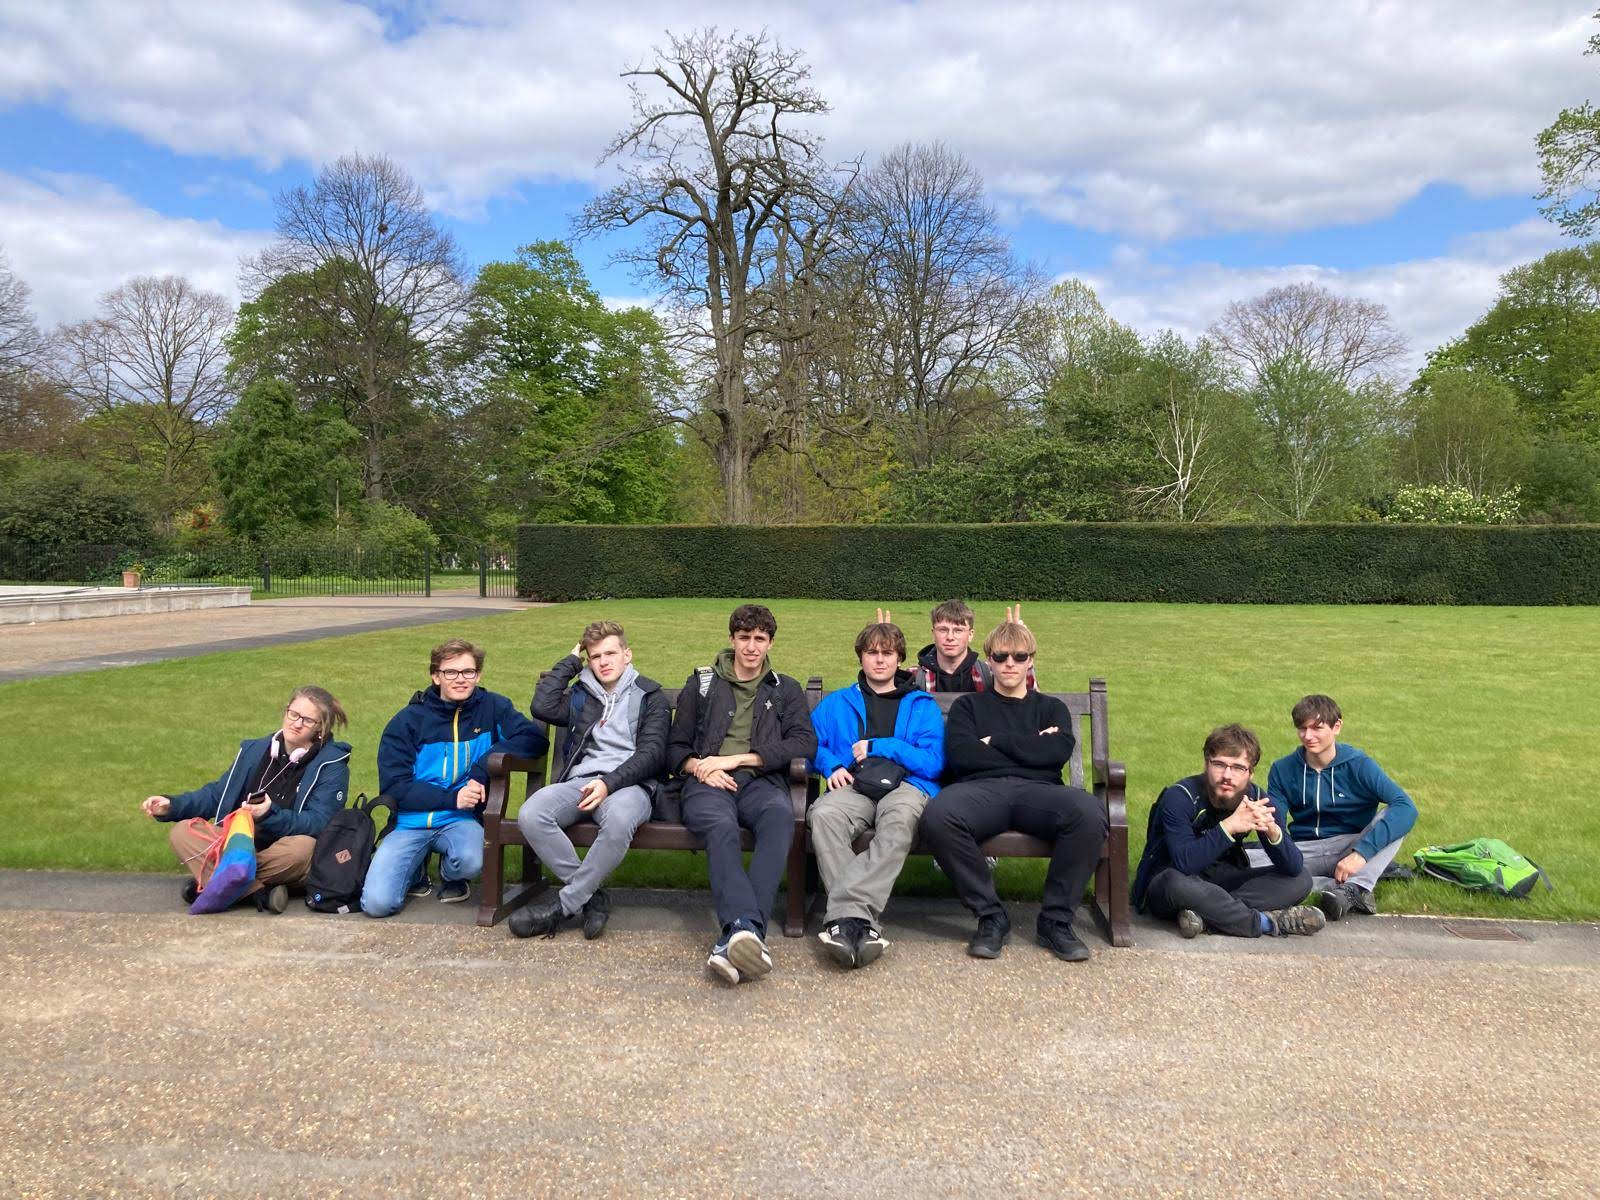
\includegraphics[width=\linewidth]{londyn.jpg}
  \end{minipage}
\end{minipage}
\newline
\noindent
\begin{minipage}{\linewidth}
  \vspace{0.75em}
  \begin{minipage}{0.32\linewidth}
    \centering \textcolor{white}{Krásné výhledy v Tatrách.}
  \end{minipage}
  \hfill
  \begin{minipage}{0.32\linewidth}
    \centering \textcolor{white}{Pohoda na vodě.}
  \end{minipage}
  \hfill
  \begin{minipage}{0.32\linewidth}
    \centering \textcolor{white}{Občas jezdíme i jinam -- naši v Londýně.}
  \end{minipage}
\end{minipage}
}

\podnadpis{MIMOŠKOLNÍ AKTIVITY}{red}
\begin{itemize}[leftmargin=10pt]
	\item \textbf{Česká středoškolská unie (ČSU)} zastupuje a hájí zájmy českých středoškoláků/středoškolaček, podporuje všeobecné vzdělávání, metodickou pestrost a inovace ve výuce, zasazuje se o zlepšování vzdělávací soustavy jako celku
	\item \textbf{Soutěž a podnikej} je organizace nabízející životní příležitost rozvinout svůj nápad v reálný podnikatelský záměr
	\item \textbf{Yoda mentorship} rozvíjí nadané a aktivní středoškoláky/středoškolačky prostřednictvím individuálního mentoringu
	\item \textbf{Bakala foundation} podporuje studium talentovaných studentů na prestižních zahraničních univerzitách
	\item \textbf{Školní sbor} zkouší každé úterý po konci vyučování a pravidelně hraje na slavnostech školy či jiných významných událostech, přihlásit se do něj může kdokoliv, kdo umí zpívat (ono by se na to stejně přišlo)
	\item \textbf{Hudebna jako zkušebna} -- Ať už si chceš založit fungl novou kapelu nebo si jen zahrát, můžeš se domluvit s profesorkou Ambrozovou, která tobě a tvojí partě ráda půjčí klíče od hudebny, kde je plno nástrojů, a budete tak moct po vyučování zkoušet!
\end{itemize}

\newpage

\nadpis{FORMÁLNÍ ZÁLEŽITOSTI}{blue}{white}{-2.5cm}

\noindent \podnadpis{JÍDELNA}{blue}
V přízemí máme samozřejmě \textbf{jídelnu}. V ní je každý školní den na výběr ze tří obědů, zpravidla dvou teplých jídel a jednoho salátu v krabičce. Ceny se pohybují v rozmezí \textbf{42 až 52 korun} (ovšem záleží na věku), v ceně je i polévka a pití.

\begin{itemize}[leftmargin=10pt]
	\item \textbf{objednávat lze dvěma způsoby}: nejlepší je, když půjdeš na \textit{jidelna.jaroska.cz} a objednáš si tam, máme ale i fyzickou \uv{narážečku} před jídelnou, kde se naskenuješ čipem a můžeš objednávat
	\item \textbf{nejzažší termín} pro objednání oběda je \textbf{do 10 hodin} předchozího pracovního dne (takže oběd na pondělí si musíš objednat už v pátek ráno)
\end{itemize}

\podnadpis{BURZA}{blue}
Stejný termín jako přihlášení obědů má i \textbf{odhlášení obědů}. Pokud onemocníš, \textbf{můžeš odhlásit oběd taky nejpozději do 10 hodin} předchozího pracovního dne. Pokud to nestihneš, můžeš ho pořád hodit do burzy. Pokud si oběd zapomeneš objednat, můžeš zkusit štěstí tady. Jestli si někdo tebou odhlášený oběd koupí, zaplatí peníze místo tebe. Pokud ne, zaplatíš je ty.

\parskip

\boxik{blue}{white}{\textbf{Pozor!} Na naší škole platí následující úsporné opatření. Stát normálně dotuje velkou část ceny oběda. Pokud si ho ale opakovaně koupíš a následně nevyzvedneš, budeš muset zaplatit plnou cenu!}

\podnadpis{OBĚDVÁNÍ}{blue}
Jídelnu máme denně otevřenou \textbf{od 11.20 do 14.00}. V téhle době si o vytyčené přestávce (vedení si na tom dost zakládá) můžeš vyzvednout svůj oběd. Pro bezkonfliktní předání doporučujeme být v \textbf{přezůvkách} (na to jsou kuchařky fakt háklivé). Batoh a bundu si nechej v nových držácích před jídelnou. \textbf{Vstoupíš dveřmi na konci chodby}, vezmeš si tácek, příbor, můžeš přibrat cestou i pití s polévkou. U výdeje se pípneš čipem a po vydání obědu už je čas zmizet ke stolu.

\parskip

\boxik{blue}{white}{\textbf{Náš tip.} V případě úplně nejhoršího scénáře, kdy si zapomeneš objednat jídlo a v burze nic není, můžeš zkusit dojít čtvrt hodiny před druhou a hodit na kuchařky psí oči, třeba ti něco dají. A i když se nevyvede s hlavním chodem, většinou ti dovolí vzít si polévku (ale od nás to nemáš!).}

\podnadpis{ZAPOMENUTÝ ČIP}{blue}
To se taky stává. Nic se neděje, stačí v průběhu dopoledne \textbf{dojít za paní
	sekretářkou}. Ta ověří tvoji volbu oběda v systému, vypíše ti \textbf{příslušný lísteček
	a tím se prokážeš} v jídelně.

\pagebreak

\polonadpis{II. Formální záležitosti}{blue}{white}{-3.8cm}

\podnadpis{ABSENCE}{blue}
Nebudeme to okecávat. Tady je flowchart, který je lepší než tisíc slov. \\
\noindent Jak si můžeš všimnout, není tady žádný rozdíl mezi nezletilým/nezletilou a zletilým/zletilou studentem/studentkou -- oficiálně zletilému/zletilé studentovi/studentce absence omlouvá pořád rodič.
%\vfill
\begin{center}
	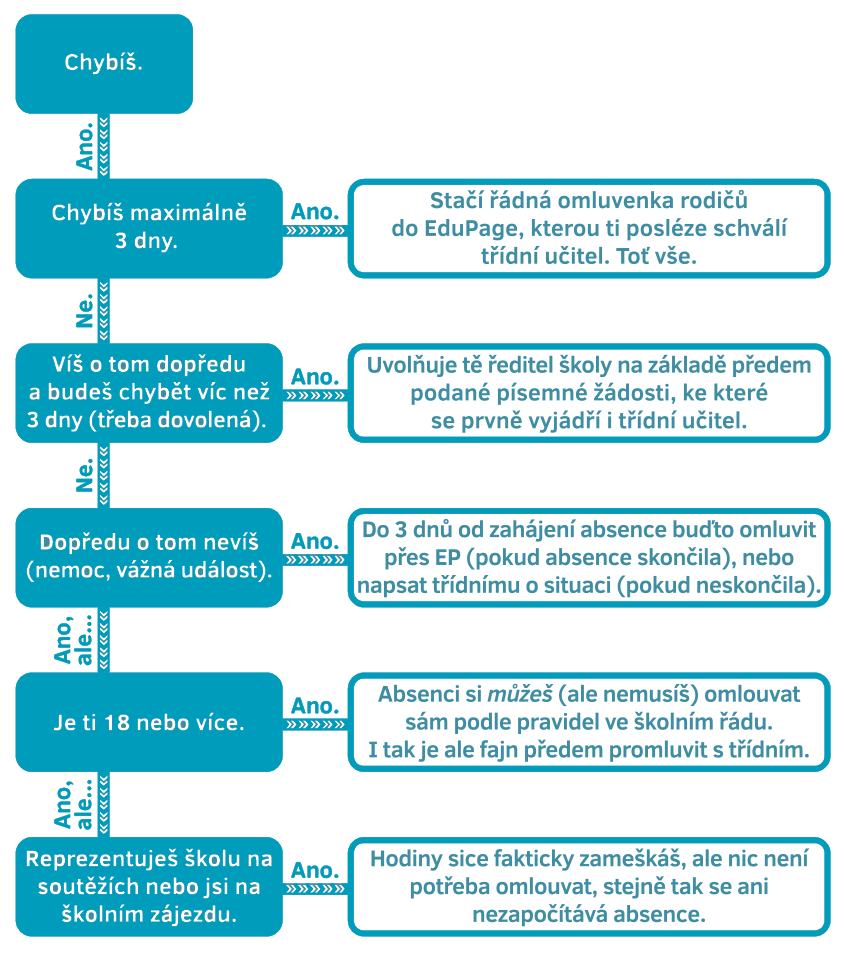
\includegraphics[width=\linewidth]{absence.png}
\end{center}

\vspace{3em}
\pagebreak

\polonadpis{II. Formální záležitosti}{blue}{white}{-3.8cm}

\podnadpis{ZNÁMKOVÁNÍ}{blue}
Každý učitel/ka má vymyšlené své způsoby známkování. \textbf{Většina se drží u staré dobré škály 1--5}, někteří ale dávají body a jiní zase procenta. Kvůli českým zákonům se ale \textbf{ve výsledku vše převede na klasické známky} (a proto nejenže budeš u těchto \uv{alternativních} systémů poučen, kolik procent je jaká známka, ale \textbf{všichni učitelé/učitelky} v září mají \textbf{povinnost poslat na EduPage pravidla klasifikace}).

\parskip

\boxik{blue}{white}{\subsection*{EDUPAGE (většinou jen EP)}
  \textbf{Naše elektronická třídnice.} Zavedli jsme ji na začátku roku 2020, takže \textbf{prošla doslova zkouškou ohněm} -- a úspěšně (i když to je diskutabilní). Občas na EP nadáváme, ale to snad ani
  nejde jinak. \\
  Faktem je, že tam najdeš \textbf{úplně všechno} -- rozvrhy, suplování, úkoly, hlasování, známky, absence, prezentace, ... A to všechno na kvadrát. \\
  A taky si tam můžeš psát s učiteli/učitelkami.}

\podnadpis{INDIVIDUÁLNÍ STUDIJNÍ PLÁN (též INDIVIDUÁL či ISP)}{blue}
Když se třeba začneš angažovat v divadle, jiném umění, či sportu, pochopitelně to neznamená, že tě vyhodíme. Na stránkách školy najdeš \textbf{tři lejstra}, která musíš pro získání individuálního studijního plánu vyplnit a předat třídnímu učiteli/učitelce. Ten to předá řediteli, který posoudí oprávněnost nároku.
ISP nemusí dávat podmínky pro úplně všechny předměty. Bohatě stačí, když se
s \textbf{jednotlivými kantory/kantorkami domluvíš} na tom, jak se bude klasifikovat. Ustálená praxe pro studenty/studentky na ISP je taková, že si \textbf{jednou za čtvrtletí docházejí napsat opakovací testy} z jednotlivých předmětů.

\parskip

\boxik{blue}{white}{\subsection*{OMLUVENÍ Z TĚLOCVIKU}
  To by jen tak nešlo. Nejdřív ti \textbf{doktor/ka musí vydat nějaké lejstro} či potvrzení o tom, že do toho tělocviku prostě nemůžeš chodit, pak ho předáš nám a... jsi omluven/a. Bude tam ještě trocha papírování, ale snažíme se vycházet vstříc (nebudeme, proboha, nikoho nutit cvičit se sádrou). V prváku také podstupujeme \textbf{test plavecké zdatnosti}, kterému se nevyhneš bez uvolnění. Pokud na něj v prváku nepřijdeš, půjdeš ve druháku. Tak důslední jsme. (Pokud nepřijdeš v druháku, přijdeš ve třeťáku. Pokud nepřijdeš ve třeťáku a zvolíš si vodácký kurz, budeš zkoušky provádět na místě před všemi svými spolužáky/spolužačkami.)}

\podnadpis{A CO JINAK?}{blue}
\textcolor{black}{\Kapitan Průvodce prváka} tady bohužel není od toho, aby poskytnul vyčerpávající výčet takovýchhle situací. Pokud nebudeš něco vědět, \textbf{prostě zajdi za třídním/třídní}. Vždycky všecko vyřeší. Ne nadarmo jim říkáme matky / otcové třídní.

\newpage

\nadpis{SOUTĚŽE}{green}{white}{-4.7cm}

\noindent Jestli je na Jarošce něco extrémně pozitivní, je to fakt, že tě \textbf{nechá dělat věci navíc} (a často tě v nich dokonce podporuje). Rozhodli jsme se tedy zkompilovat \textbf{seznam soutěží a jiných aktivit}, které ti zdejší studium umožňuje.

\podnadpis{STŘEDOŠKOLSKÁ ODBORNÁ ČINNOST (SOČ)}{green}
SOČka představuje možnost zkusit už na střední škole \textbf{dělat opravdovou vědu}. Cílem SOČky je provést vlastní výzkum a získané poznatky \textbf{prezentovat před náročnou komisí}. Výběr okruhů bývá dostatečně široký, najdeš témata jak technicky, tak humanitně zaměřená. Navíc ji můžeš použít jako závěrečnou práci, kterou musí všichni napsat ve třetím ročníku.

\podnadpis{PŘEDMĚTOVÉ OLYMPIÁDY}{green}
Matematika, fyzika, biologie, chemie, zeměpis, dějepis, český jazyk, ekologie. To je základní paleta předmětových olympiád, ve kterých u nás můžeš zkusit štěstí. V olympiádách najdeš typicky k řešení úlohy složitější, než jsou ty běžně řešené v hodinách. Pro úspěch v nich je potřeba mít komplexní znalosti v daném oboru. Přehled těchto olympiád a dalších soutěží je k mání na \textit{chces-soutezit.cz}.

\podnadpis{T-EXKURZE}{green}
Dvakrát do roka si vybraná vysokoškolská pracoviště pozvou středoškoláky/středoškolačky do svých laboratoří, kde si mohou vyzkoušet, jak se dělá reálná věda. Přihlášení je jednoduché: stačí vyplnit pár otázek na dané téma a připojit motivační dopis (a občas ani to ne). Stojí to za zvážení!
\par \noindent Níže pak už najdeš jen výčet dalších soutěží dle kategorií (který určitě není vyčerpávající). Jejich hlavní cenou je obvykle dobrý pocit nebo možnost účasti na \textbf{dedikovaném soustředění}, kde se můžeš setkat s obdobně divnými lidmi jako jsi ty sám. Jednotlivé soutěže se liší jak obtížností, tak časovou náročností. Každý si tak může najít svoji optimální, do které se mu bude chtít investovat energie.

\begin{multicols}{3}
	\footnotesize
	\noindent\textcolor{green}{Matematika:}
	\begin{itemize}[leftmargin=10pt]
		\item BrKoS
		\item MaSo
		\item KoMár
		\item Matematický náboj
		\item Mathrace
		\item Prase
	\end{itemize}
	\textcolor{green}{Chemie:}
	\begin{itemize}[leftmargin=10pt]
		\item VíBuCh
		\item Chemiklání
		\item Ksicht
	\end{itemize}
	\vfill\null\columnbreak
	\textcolor{green}{Biologie:}
	\begin{itemize}[leftmargin=10pt]
		\item Biozvěst
		\item IBIS
	\end{itemize}
	\textcolor{green}{Informatika:}
	\begin{itemize}[leftmargin=10pt]
		\item FIKS
		\item MOROUS
		\item Ksicht
		\item IKS
	\end{itemize}
	\vfill\null\columnbreak
	\textcolor{green}{Fyzika:}
	\begin{itemize}[leftmargin=10pt]
		\item Fykos
		\item Fyziklání
		\item Fyzikální náboj
		\item TSAF, DSEF, VAG
	\end{itemize}
	\textcolor{green}{Šifrovačky:}
	\begin{itemize}[leftmargin=10pt]
		\item Tmou, Dnem
		\item BrLoH
		\item Intersob, Interlos
		\item LamoLamy
	\end{itemize}
	\vspace*{1em}
\end{multicols}

\normalsize
\pagebreak

\nadpis{ZA HRANICEMI ŠKOLY}{yellow}{white}{-2.75cm}

\enlargethispage{\pagegoal}
\noindent \small Ano, víme, na Jarošce je fajn! Ale kam si po ní jít vyčistit s kamarády/kamarádkami hlavu nebo kde najít inspirativní prostředí na projekt? Na to máme \textbf{skvělé kavárny v okolí}. A~že jich je! Připravili jsme si tady výčet těch nejlepších (a na další dvojstránce máme jejich podrobnou mapku, abys trefil/a i potmě).\\

\noindent
\begin{minipage}{0.7\textwidth}
	\podnadpis{MILADY KAFFEE}{yellow}
	\textcolor{yellow}{Po--Pá: 7:30--20 hod $\bullet$ So, Ne: 9--20 hod}
	\vspace{5pt}
	\small
	\begin{itemize}[leftmargin=10pt]
		\item \textbf{2 minuty} pěšky
		\item značka kávy: \textbf{Coffee Collective} (z Dánska), \textbf{The Space Coffee} (z Brna)
		\item všechno jídlo je \textbf{vegetariánské}
		\item v létě mají \textbf{zahrádku} a každý rok je tu \textbf{blešák} (viz FB)
		\item obsluha doporučuje \textbf{caprese sendvič} s domácím pestem
	\end{itemize}
\end{minipage}
\hfill
\begin{minipage}{0.27\textwidth}
	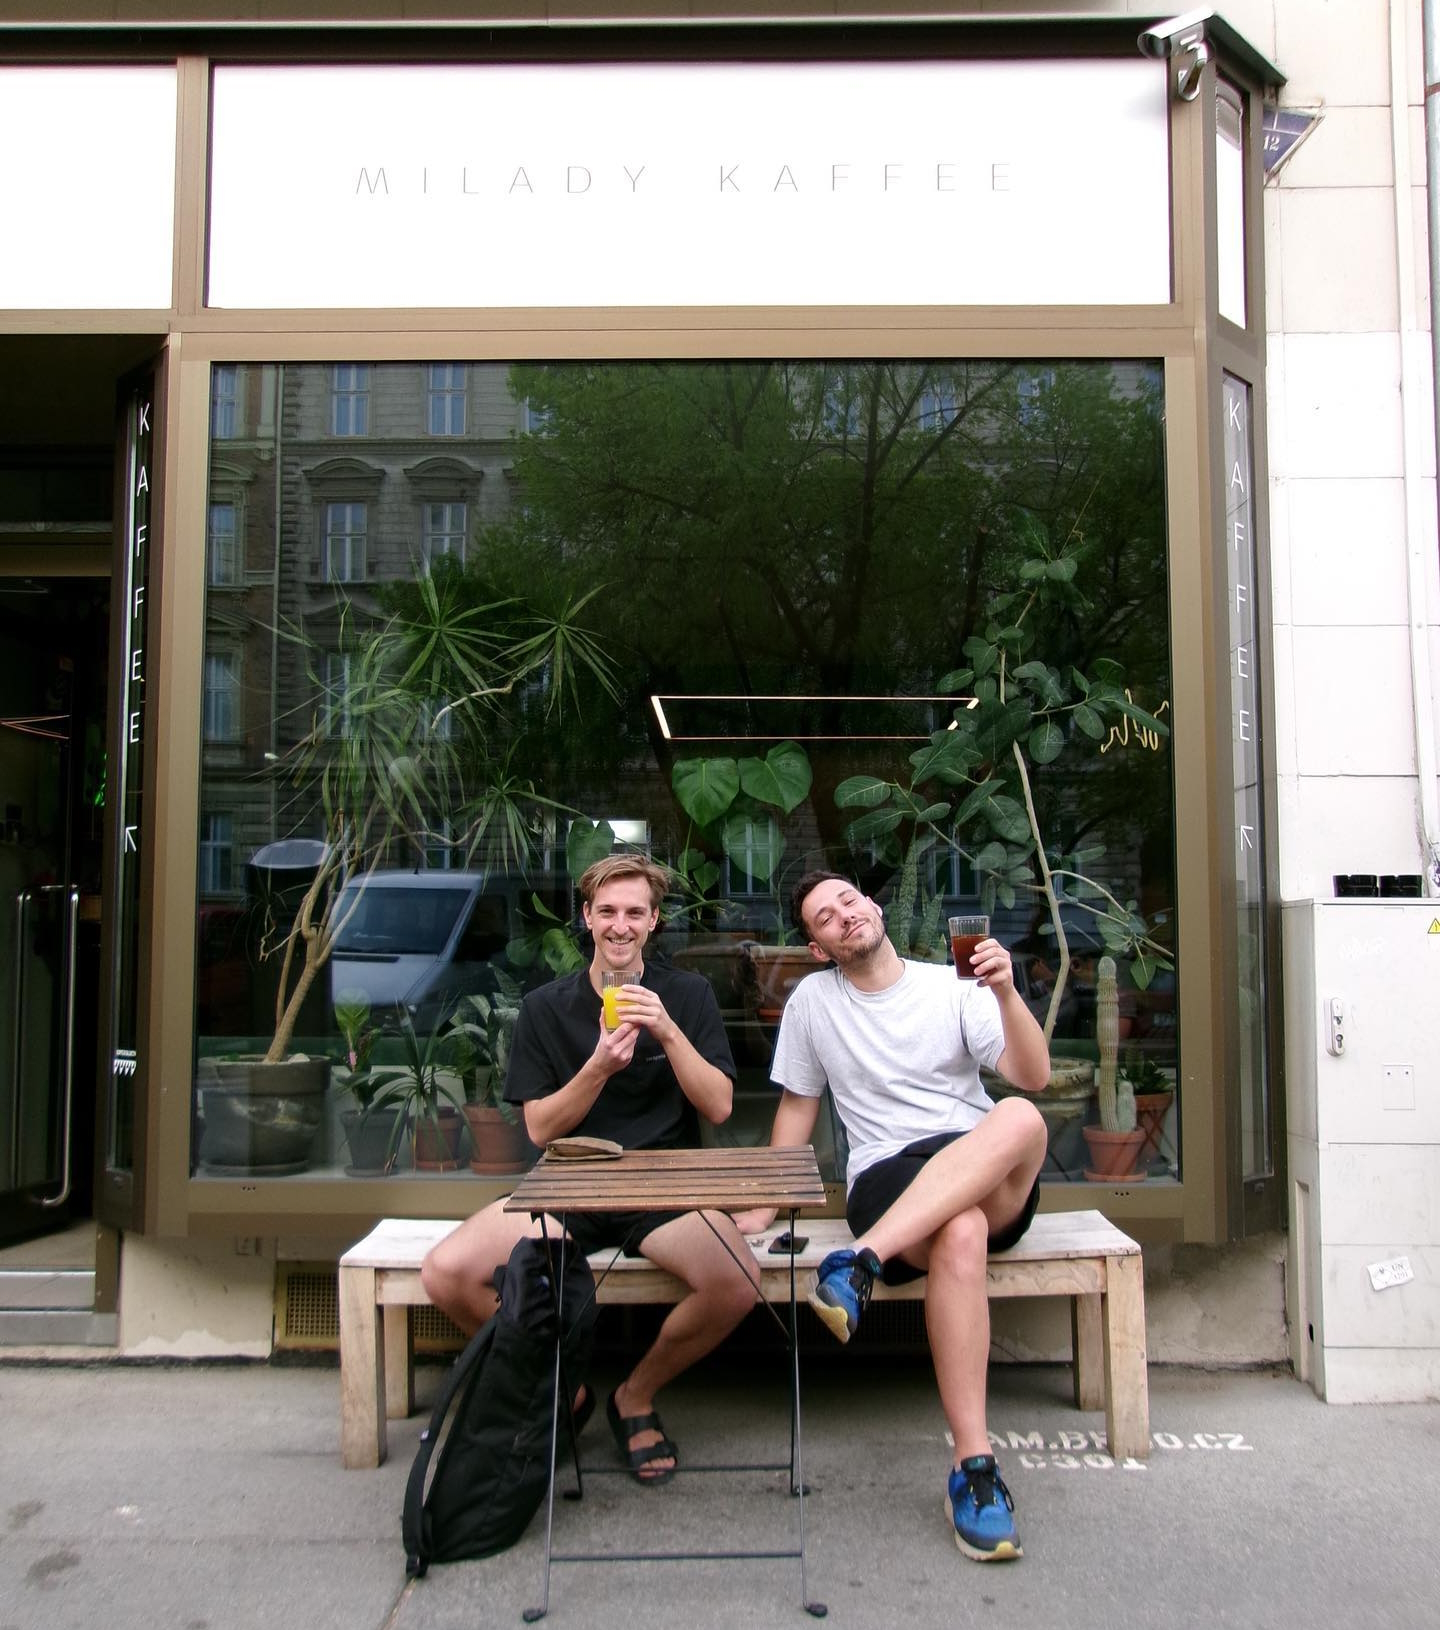
\includegraphics[width=\linewidth]{milady_kaffee.jpg}
\end{minipage}
\\

\boxik{yellow}{white}{
  \begin{minipage}{0.27\textwidth}
    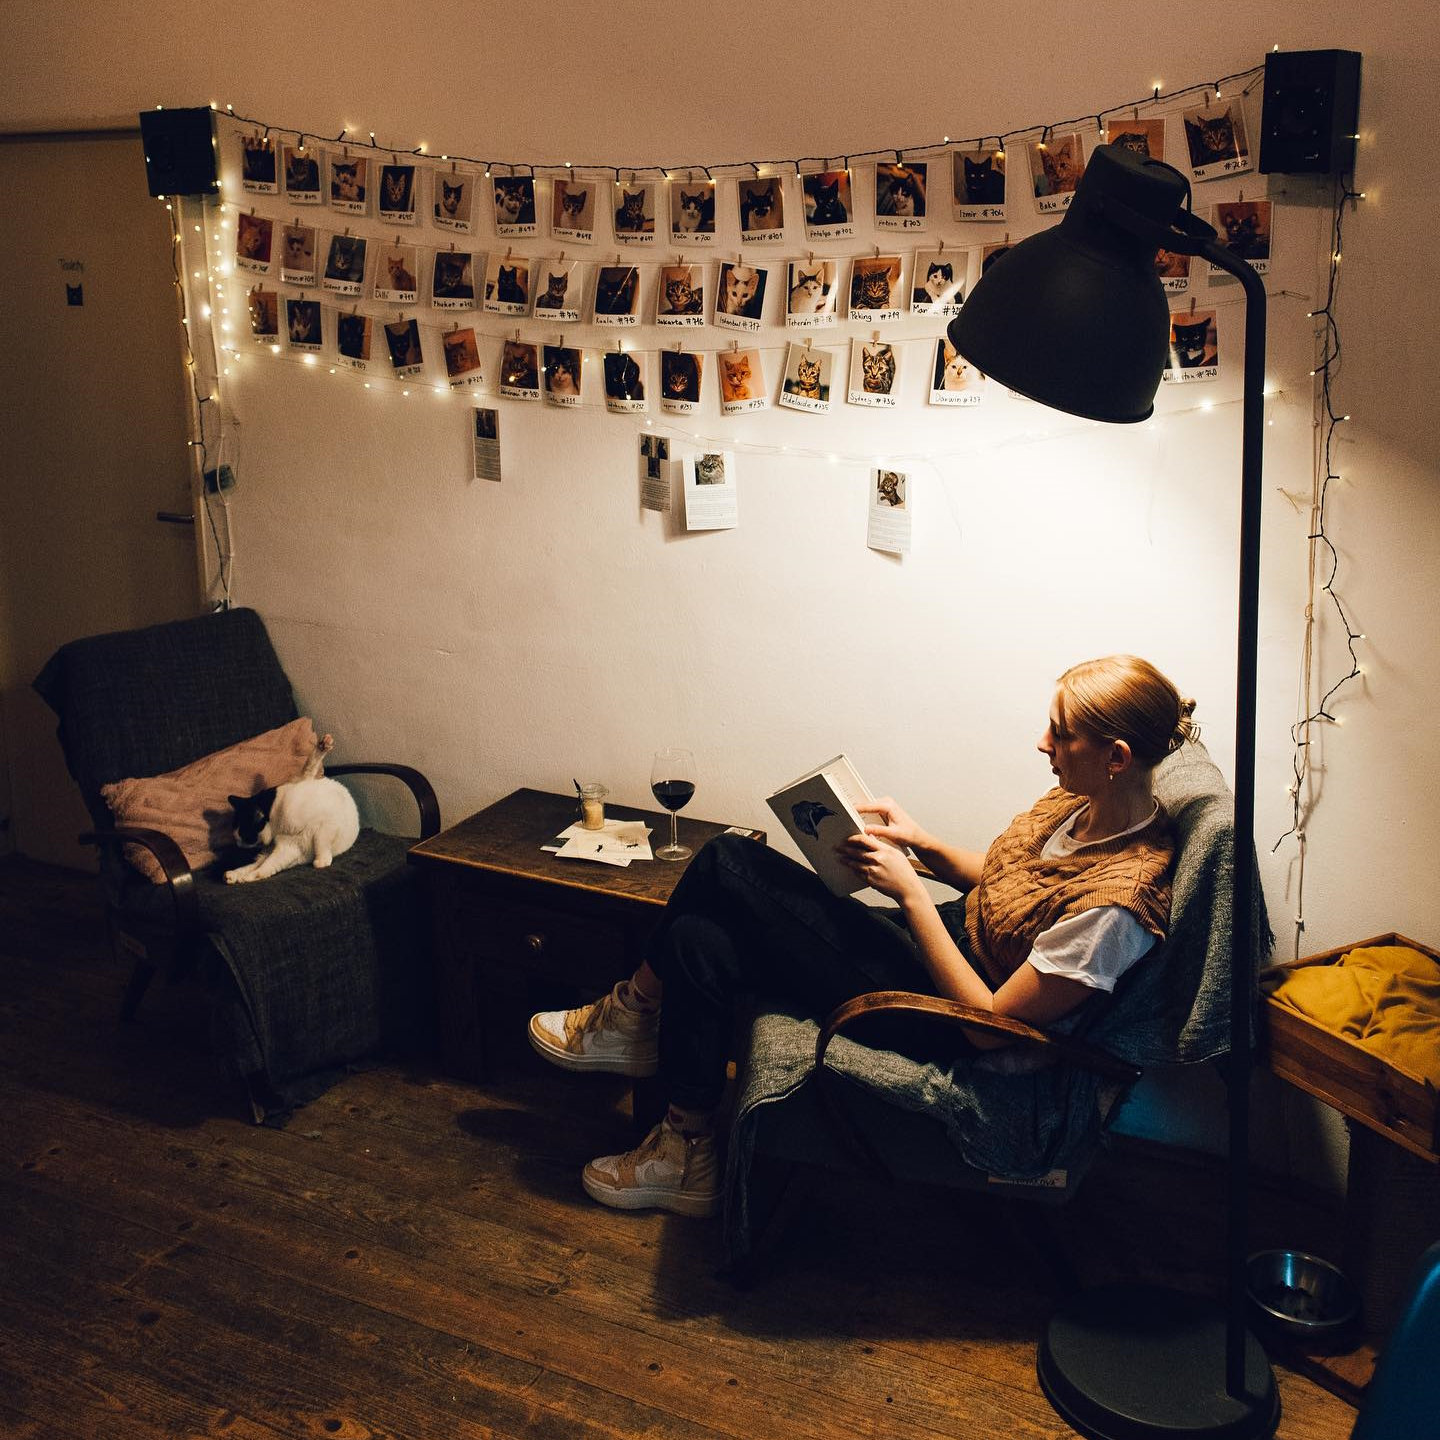
\includegraphics[width=\linewidth]{pelisek.jpg}
  \end{minipage}
  \hfill
  \begin{minipage}{0.7\textwidth}
    \vspace{-5pt}
    \textcolor{white}{
      \subsection*{PELÍŠEK -- kočičí kavárna}
      Po--Pá: 10--21 hod $\bullet$ So, Ne: 13--19 hod
      \small
      \begin{itemize}[leftmargin=10pt]
        \item \textbf{3 minuty} pěšky
        \item značka kávy: různí se, hlavně \uv{\textbf{mini pražírny}}
        \item \textbf{super na práci a učení} (pokud sneseš kočky)
        \item \textbf{je veganský}, najdeš tam veganské toasty i dezerty
        \item kteroukoli tamější kočičku si \textbf{můžeš adoptovat}
        \item obsluha doporučuje \textbf{espresso s višňovým tonicem} a \textbf{naked dorty}
      \end{itemize}
    }
  \end{minipage}
}

\noindent \begin{minipage}{0.7\textwidth}
	\podnadpis{COFFEE TRAIL}{yellow}
	\textcolor{yellow}{Po--Pá: 8--20 hod $\bullet$ So, Ne: 9--16 hod}
	\vspace{5pt}
	\small
	\begin{itemize}[leftmargin=10pt]
		\item \textbf{7 minut} pěšky
		\item značka kávy: \textbf{Fifty Beans} (brněnská pražírna)
		\item mají velký výběr \textbf{snídaní} a denně jiné \textbf{polévky}
		\item chleba odebírají z \textbf{Chleba Brno} a jsou všeobecně bio
		\item obsluha doporučuje \textbf{banana bread}
	\end{itemize}
\end{minipage}
\hfill
\begin{minipage}{0.27\textwidth}
	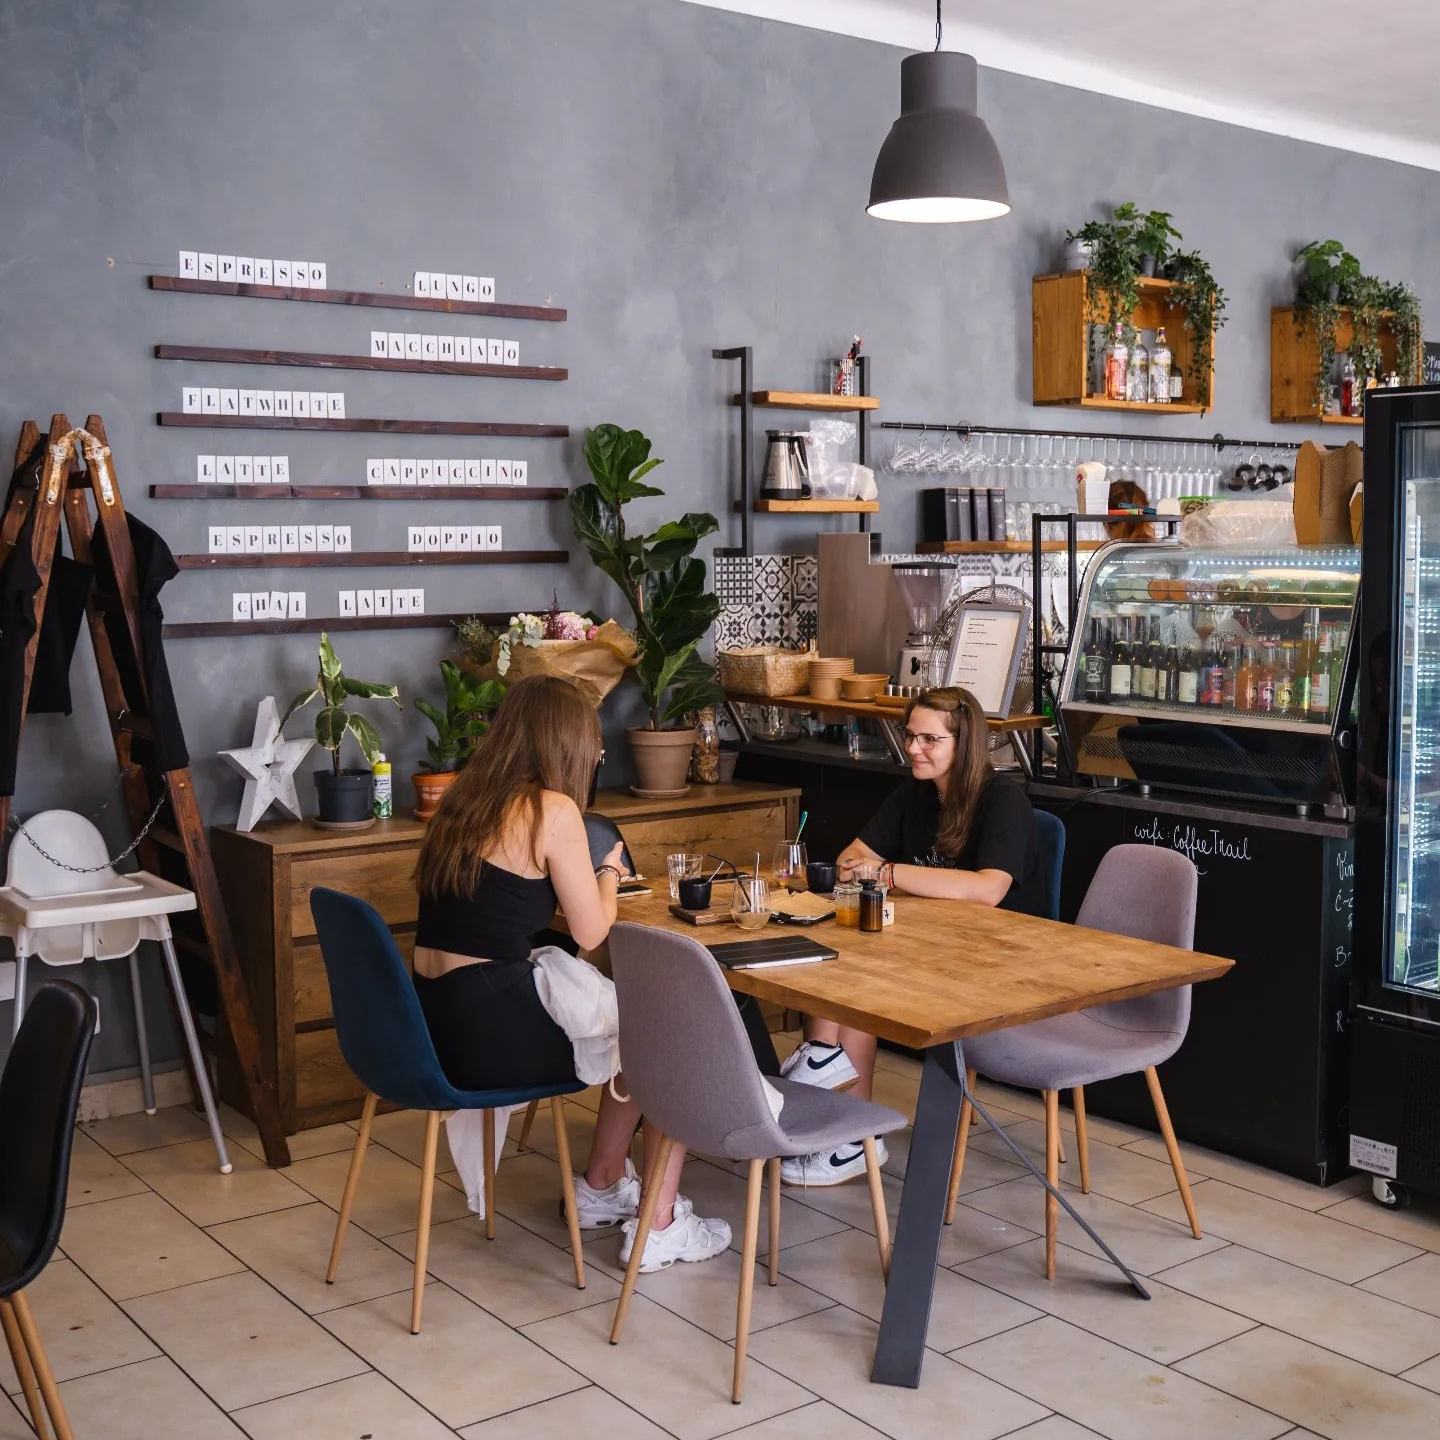
\includegraphics[width=\linewidth]{coffee_trail.jpg}
\end{minipage}

\boxik{yellow}{white}{
  \begin{minipage}{0.23\textwidth}
    \vspace*{-8em}
    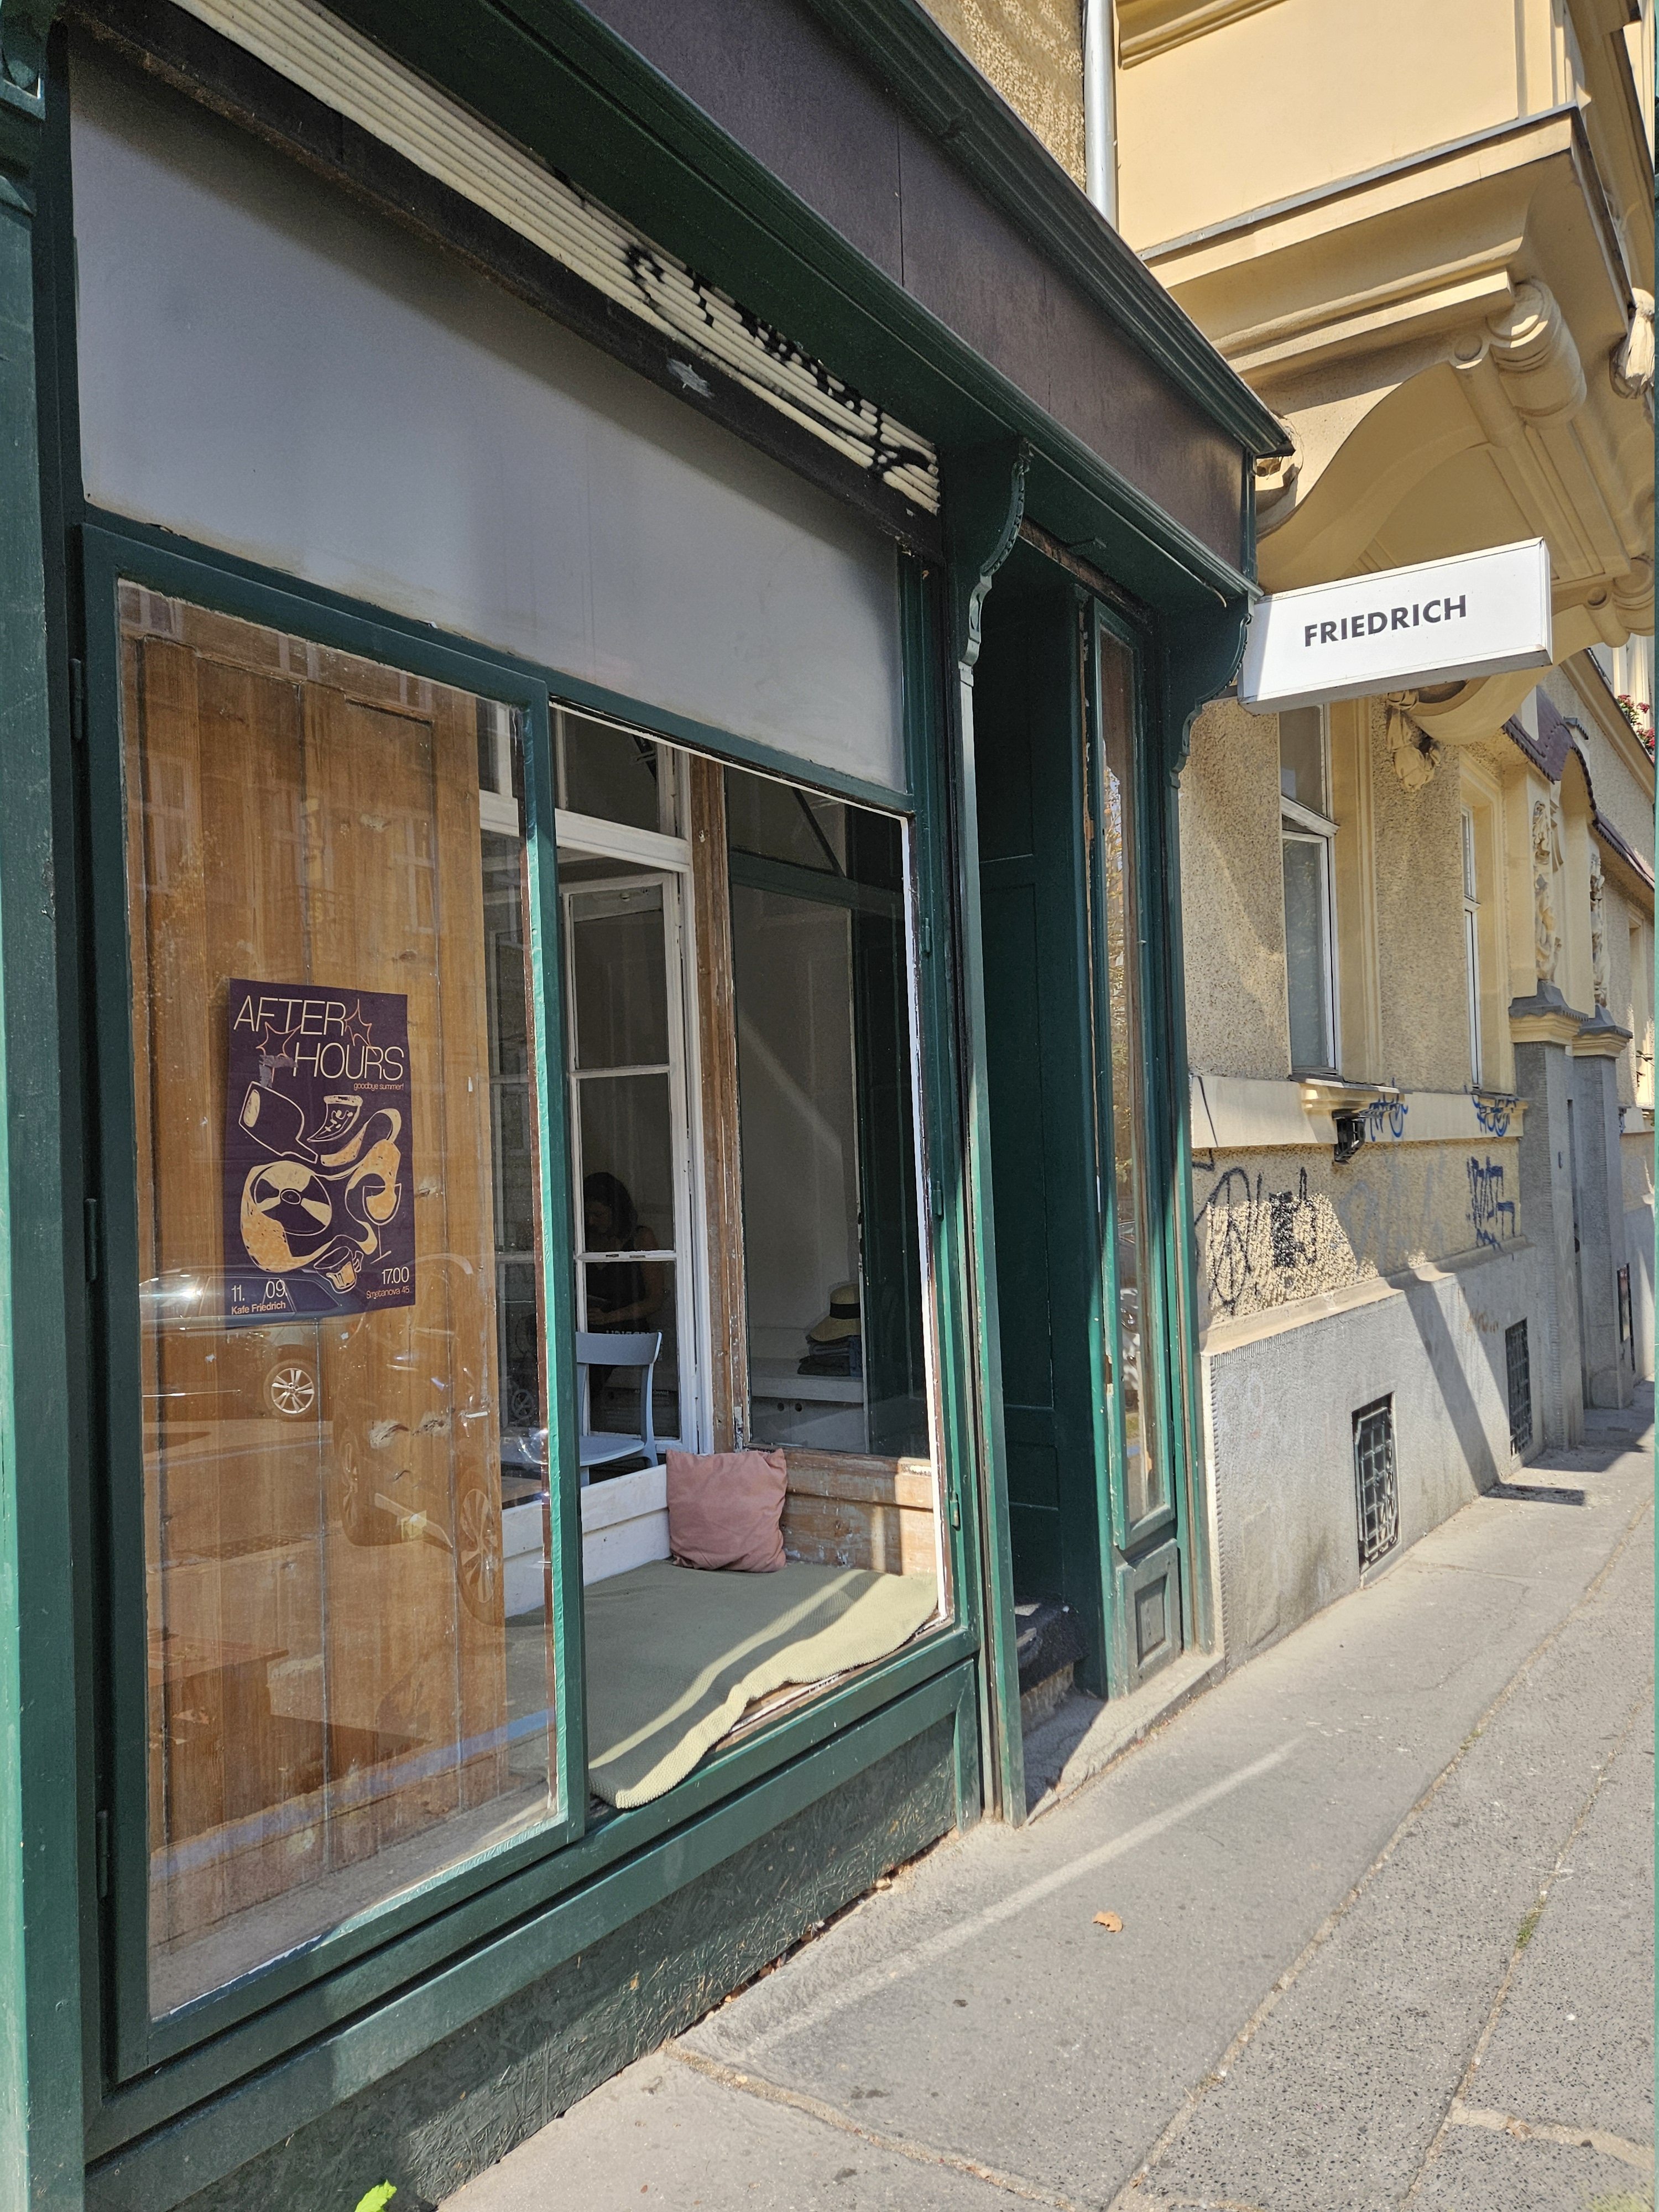
\includegraphics[width=\linewidth]{friedrich.jpg}
  \end{minipage}
  \hfill
  \begin{minipage}{0.7\textwidth}
    \vspace{-5pt}
    \textcolor{white}{
      \subsection*{KAFE FRIEDRICH}
      Po--Pá: 8--20 hod $\bullet$ So: 9--19 hod $\bullet$ Ne: zavřeno
      \small
      \begin{itemize}[leftmargin=10pt]
        \item \textbf{10 minut} pěšky
        \item značka kávy: výběrová \textbf{La Cabra} (z Dánska)
        \item vše je \textbf{veganské} a \textbf{lokální}, včetně jejich skvělých brunchů
        \item Kafe Friedrich najdeš na Gastromapě Lukáše Hejlíka
        \item obsluha doporučuje \textbf{skořicové šneky}
      \end{itemize}
    }
    \vspace{10em}
  \end{minipage}
}

\pagebreak
\polonadpis{IV. Za hranicemi školy}{yellow}{white}{-3.8cm}

\noindent
\begin{minipage}{0.7\textwidth}
	\podnadpis{COFFEE BAR STORY}{yellow}
	\textcolor{yellow}{Po--Pá: 8--19 hod $\bullet$ So, Ne: 9--19 hod}
	\vspace{5pt}
	\small
	\begin{itemize}[leftmargin=10pt]
		\item \textbf{8 minut} pěšky
		\item značka kávy: \textbf{Fifty Beans} (brněnská pražírna)
		\item bohatý výběr \textbf{snídaní, brunchů a svačin} (sendviče, lívance, nebo třeba avokádový chléb)
		\item obsluha doporučuje \textbf{matchavance s omáčkou z lesních plodů}
	\end{itemize}
\end{minipage}
\hfill
\begin{minipage}{0.27\textwidth}
	\includegraphics[width=\linewidth]{mymika.jpg}
\end{minipage}

\boxik{yellow}{white}{
\begin{minipage}{0.27\textwidth}
  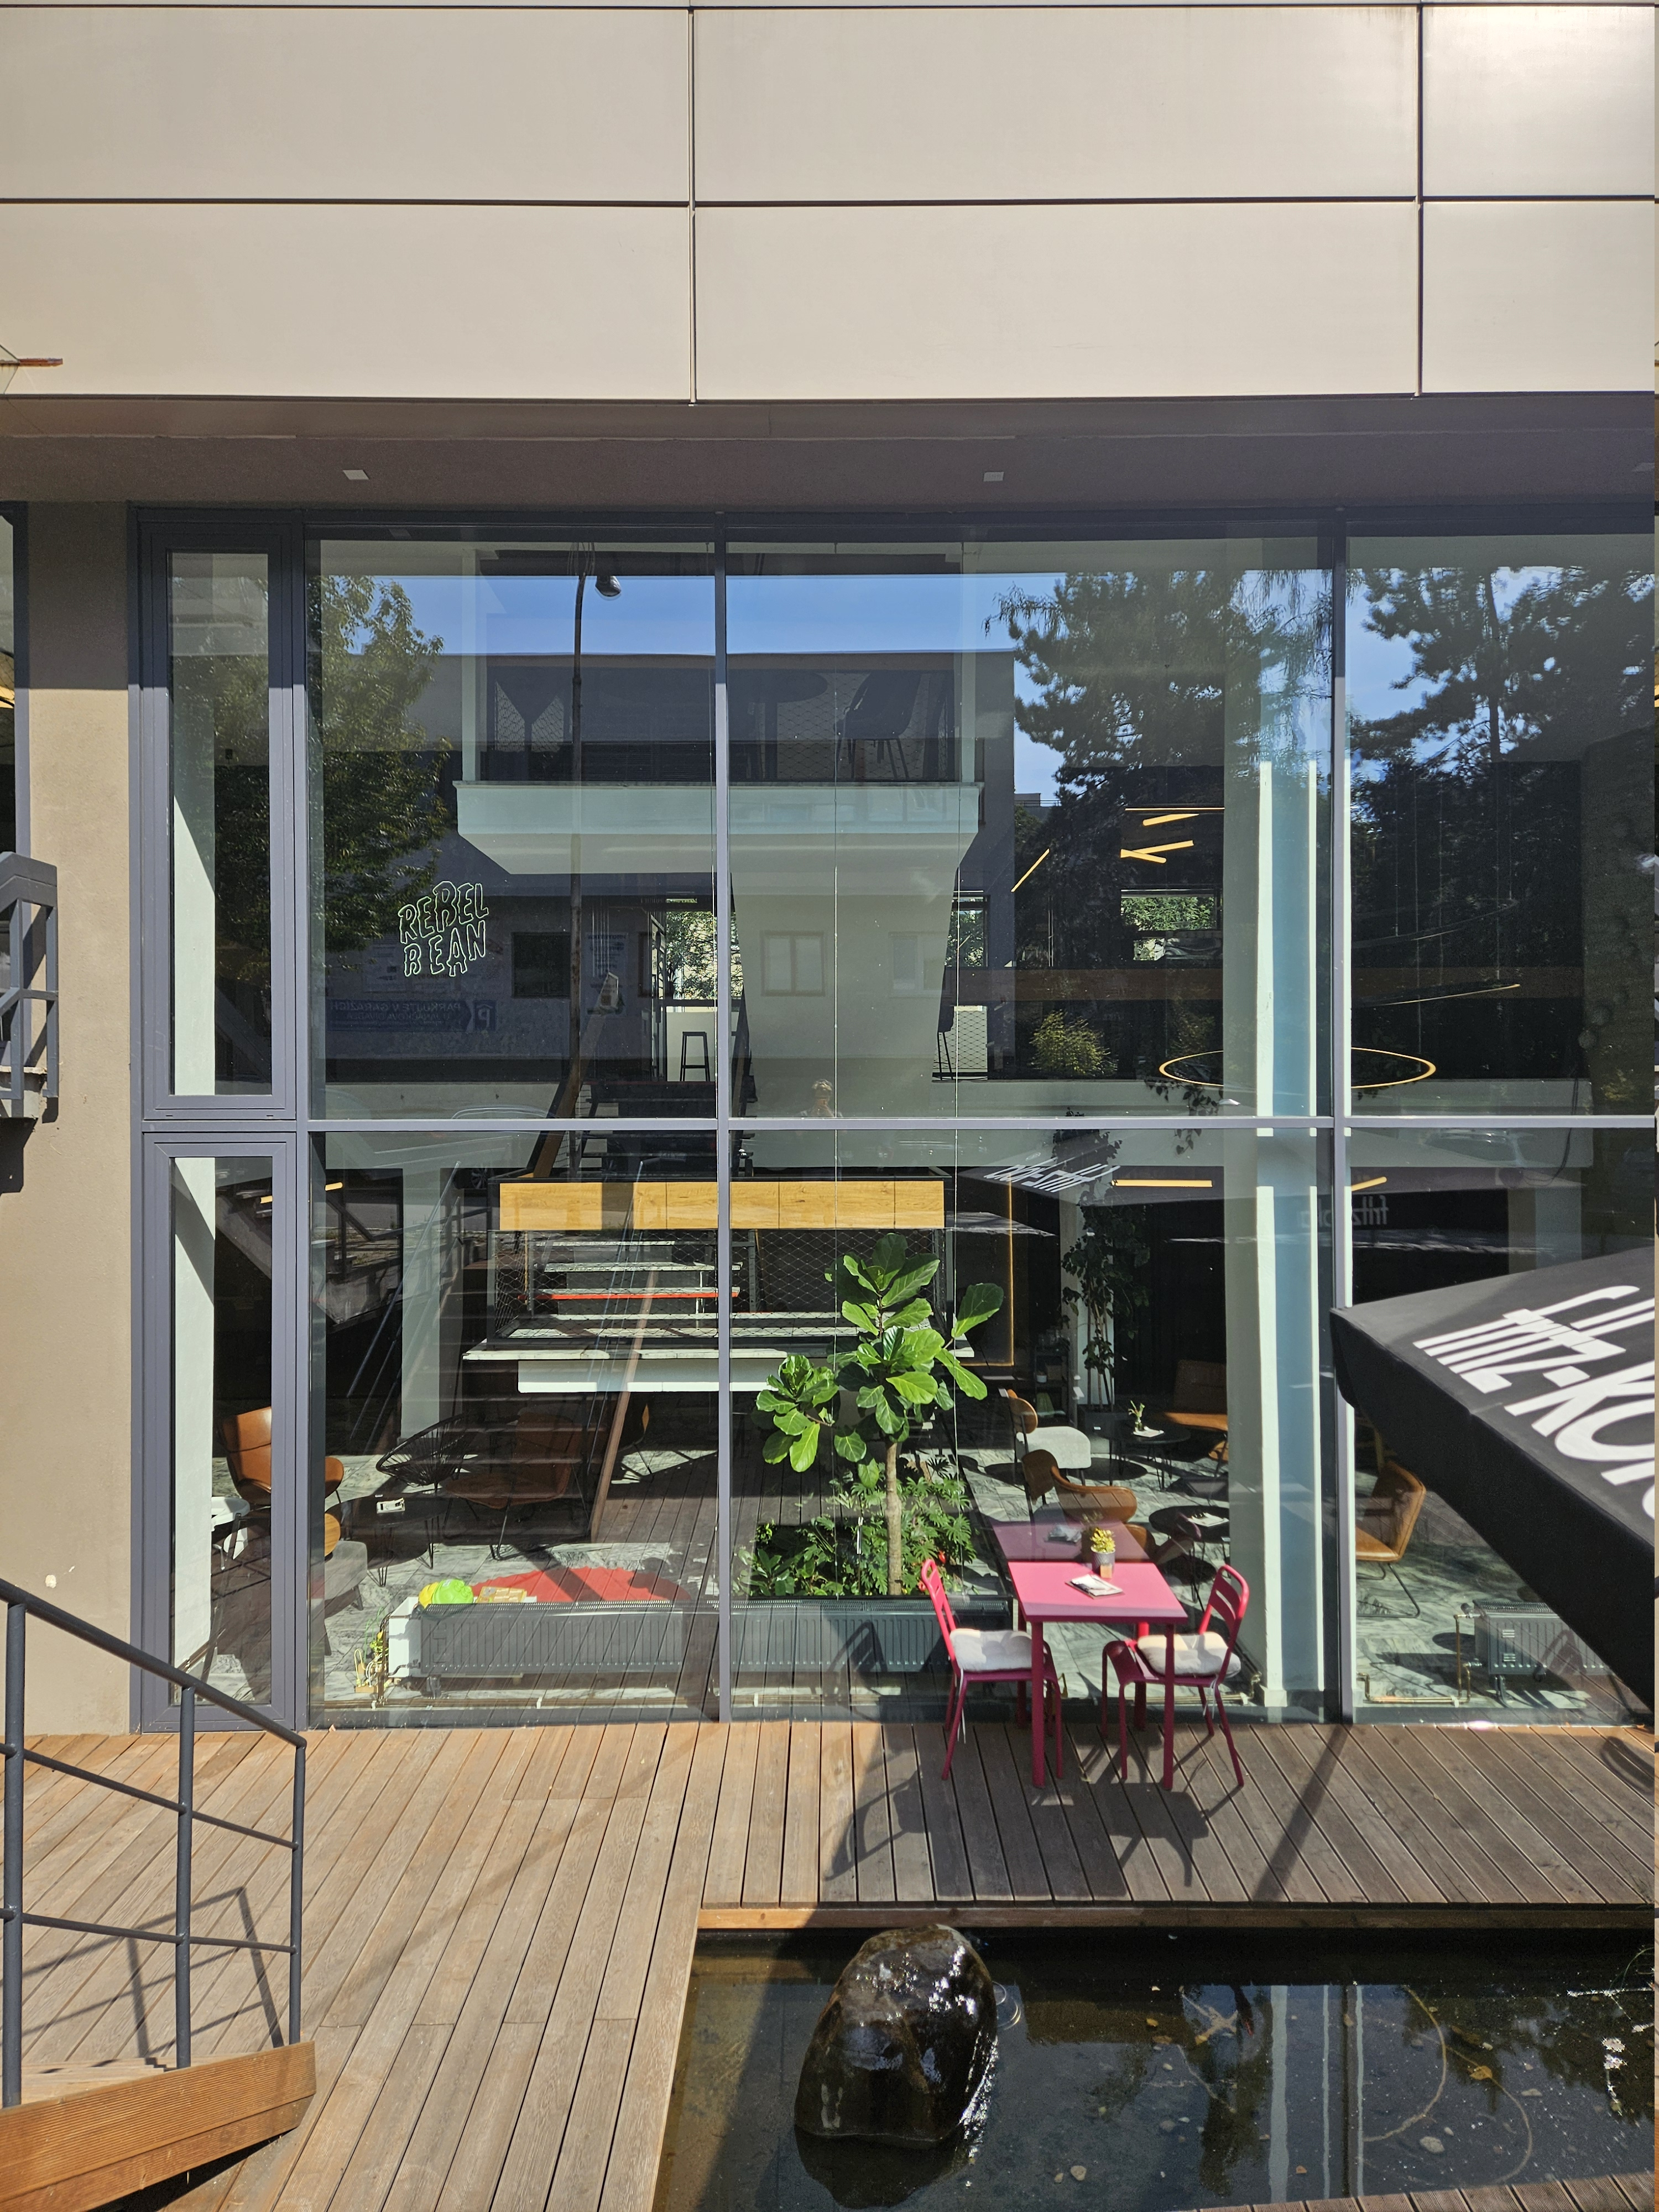
\includegraphics[width=\linewidth]{pole.jpg}
\end{minipage}
\hfill
\begin{minipage}{0.7\textwidth}
  \vspace{-5pt}
  \textcolor{white}{
    \subsection*{REBELBEAN POLE}
    Po--Pá: 7:30--20 hod $\bullet$ So, Ne: 8--20 hod
    \small
    \begin{itemize}[leftmargin=10pt]
      \item z nám. 28. října jeď jednu zastávku šalinou na Dětskou nemocnici, pak je to za rohem
      \item značka kávy: \textbf{Rebelbean} (brněnská pražírna)
      \item mají od všeho něco: výběr \textbf{snídaní}, \textbf{hot dogů} i sladkých \textbf{lívanečků}
      \item naše redakce doporučuje \textbf{zapečený toust s vejcemi}
    \end{itemize}
  }
\end{minipage}
}

\noindent\begin{minipage}{0.7\textwidth}
	\podnadpis{ANODA$^+$}{yellow}
	\textcolor{yellow}{Po--Čt: 8--23 hod $\bullet$ Pá: 8--2 hod $\bullet$ So: 10--1 hod $\bullet$ Ne: 10--22 hod}
	\vspace{5pt}
	\small
	\begin{itemize}[leftmargin=10pt]
		\item \textbf{3 minuty} pěšky (hned za Pelíškem)
		\item značka kávy: \textbf{Rusty Nails Coffee Roasters} a další
		\item jídla tolik nemají, ale jejich sendvič stojí za to
		\item zletilí studenti/studentky si mohou dát výborné pivo \textbf{Kočovný Kozi}
		\item v Anodě se párkrát do měsíce hraje \textbf{živé techno}
		\item na pití doporučuje obsluha \textbf{espresso tonic} a \textbf{kakao}
	\end{itemize}
\end{minipage}
\hfill
\begin{minipage}{0.27\textwidth}
	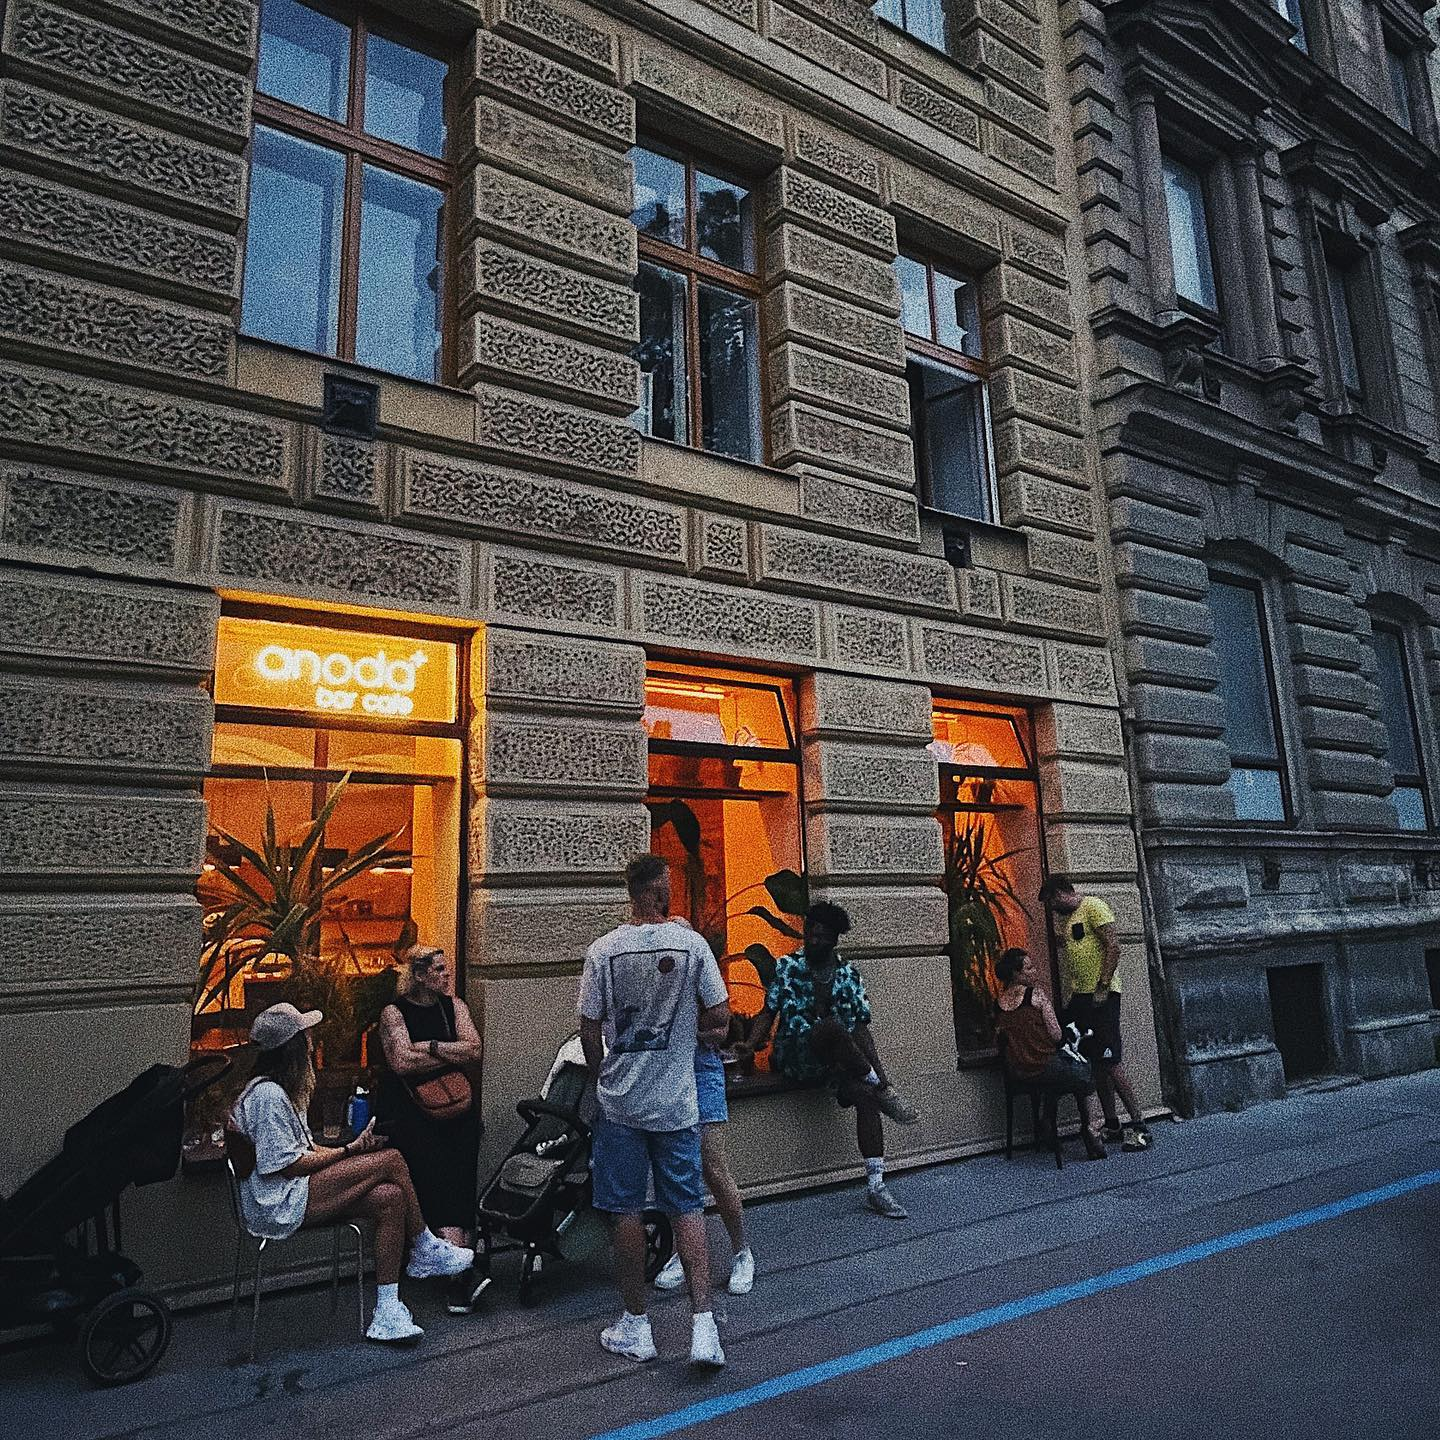
\includegraphics[width=\linewidth]{anoda.jpg}
\end{minipage}

\vfill

\podnadpis{TOBĚ TO NESTAČÍ?}{yellow}
Ještě nemáš vybráno? V okolí je ještě \textcolor{yellow}{\textbf{Park Lane}}, kde budeš mít klid a prostor na práci a učení. No a pokud zrovna nemáš chuť na kafe, ale třeba na pivo (pouze zletilí!), poblíž je spousta skvělých hospod, jako třeba \textcolor{yellow}{\textbf{Tři ocásci}}, \textcolor{yellow}{\textbf{Mýdlo}}, \textcolor{yellow}{\textbf{Traubka}} nebo \textcolor{yellow}{\textbf{Doubravník}}. Pokud sis zase zapomněl/a oběd, za obědovou přestávku se dá stihnout dojít do \textcolor{yellow}{\textbf{D\&T Marketu}}, na točenou zmrzlinu nebo smažák v housce do \textcolor{yellow}{\textbf{La Vanille}} nebo na dobré pečivo do \textcolor{yellow}{\textbf{Matějova pekařství}}, svižným krokem i do \textcolor{yellow}{\textbf{La Speranzy}}, na \textcolor{yellow}{\textbf{Kurdský kebab}} nebo do \textcolor{yellow}{\textbf{Albertu}} u Moraváku.

\pagebreak
%\begin{landscape}

\newgeometry{left=0cm,bottom=0cm,top=0cm,bottom=0cm}
\noindent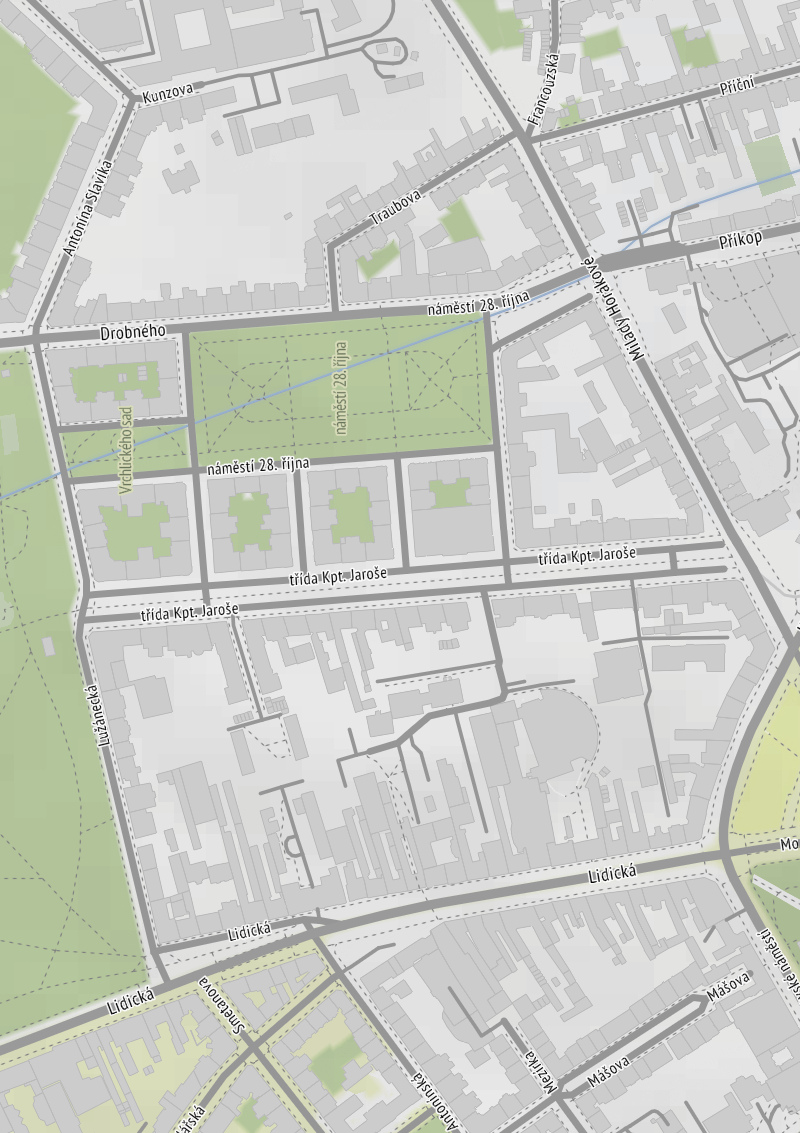
\includegraphics[width=\paperwidth]{mapa.png}
\restoregeometry
\pagebreak
%\end{landscape}

\pagestyle{empty}
\pagecolor{red}
\noindent\hspace{-3pt}\textcolor{white}{\fontsize{20}{20} \Kapitan Jaroška}

\vspace*{\fill}


\noindent\hspace{-3pt}\textcolor{white}{\fontsize{25}{25} \Kapitan Průvodce prváka. \colorbox{blue}{\rule[5pt]{0pt}{15pt}\large 2024/2025}}

\vspace{1em}

\noindent\textcolor{white}{\textbf{Vydáno Studentským parlamentem Jarošky v září 2024 nákladem 130 výtisků.}}

\vspace{1em}

\noindent \textcolor{white}{\textbf{Redakce: Dominik Doležel, Jan Romanovský}}

\vspace{1em}

\noindent \textcolor{white}{\textbf{Foto: Dominik Doležel, Hana Trubačíková, Mgr. Bc. Jaroslava Maříková, archivy institucí}}

\vspace{1em}

\noindent \textcolor{white}{\textbf{Sazba a grafická úprava: Dominik Doležel, Jan Romanovský}}

\vspace{1em}

\noindent \textcolor{white}{\textbf{Spolupráce: Mgr. Jana Sítařová, Šimon Lopour}}

\vspace{1em}

\noindent \textcolor{white}{\textbf{Účelová publikace -- výtisk je neprodejný.}}

\vspace{1em}

\noindent \textcolor{white}{\textbf{Vysázeno v \LaTeX u.}}



\end{document}
